\section{Detector Design and Hardware}\label{sec:detector}

% T. Ishida, R. Henderson, A. Konaka, Y. Kudenko, T. Lindner, S. Nakayama, Y. Nishimura, F. Retiere, M. Shiozawa, H.-K. Tanaka, M. Ziembicki, TRIUMF, ICRR

The \nuprism detector uses the same water Cherenkov detection technology as Super-K with a cylindrical water volume that is taller than Super-K (50-100m vs 41m) but with a much smaller diameter (6-10m vs 39m). The key requirements are that the detector span the necessary off-axis range (1$^\circ$-4$^\circ$) and that the diameter is large enough to contain the maximum required muon momentum. The baseline design considers a detector location that is 1~km downstream of the neutrino interaction target with a maximum contained muon momentum of 1~GeV/c. This corresponds to a 50~m tall tank with a 6~m diameter inner detector (ID) and a 10~m diameter outer detector (OD), as shown in Figure~\ref{fig:nuprismpic}. A larger, 8~m ID is also being considered at the expense of some OD volume in the downstream portion of the tank. As the \nuprism analysis studies mature, the exact detector dimensions will be refined to ensure sufficient muon momentum, \nue statistics and purity, etc.

\begin{figure}[htbp]
\centering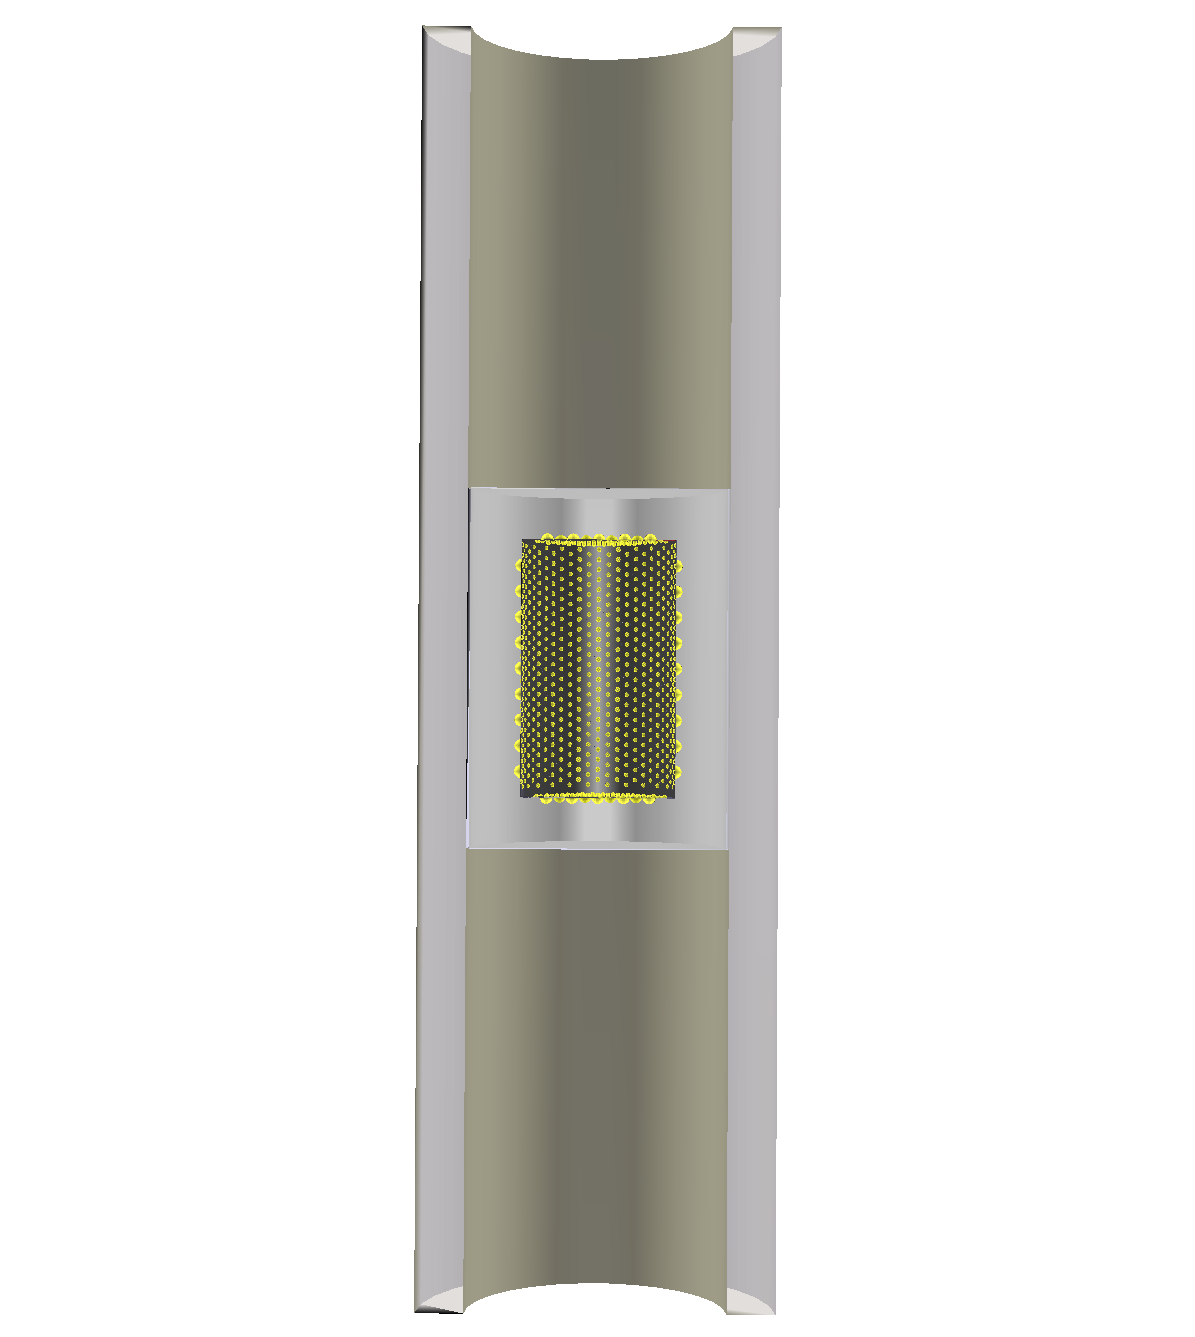
\includegraphics[width=9cm,angle=0]{figures/nuprism-middlecut.png}
\caption{The planned configuration of the nuPRISM detector within the water tank is shown. The instrumented portion of the tank moves vertically to sample different off-axis angle regions.}
\label{fig:nuprismpic} 
\end{figure}

The instrumented portion of the tank is a subset of the full height of the water volume, currently assumed to be 10~m for the ID and 14~m for the OD. The novel feature of this detector is the ability to raise and lower the instrumented section of the tank in order to span the full off-axis range in 6 steps. The inner detector will be instrumented with either 5-inch or 8-inch PMTs to ensure sufficient measurement granularity for the shorter light propagation distances relative to Super-K. Also under consideration is to replace the OD reflectors with large SMRD-style scintillator panels, as discussed in Section~\ref{sec:scint}, although this has not yet been integrated into the overall detector design.

The remainder of this section describes the elements needed for \nuprism and corresponding cost estimates, where available. The cost drivers for the experiment are the civil construction and the cost of the PMTs, and, correspondingly, more detailed cost information is presented in those sections.

%Section goals:
%\begin{itemize}
%\item Overview of hardware issues (references to associated physics studies)
%\item Mention unique requirement to raise and lower detector
%\end{itemize}


\subsection{Site Selection}

The \nuprism detector location is determined by several factors, such as signal statistics, accidental pile-up rates, cost of digging the pit, and potential sites available.
At 2.5$^o$ off-axis position at 1~km with a fiducial volume size of 4~m diameter and 8~m high cylinder, the neutrino event rate at \nuprism is more than 300 times that of SK. At 2km, the number of events drops by a factor of 4, which yields 75 times more events than SK, for the same size of the detector. The impact of the number of events collected on the physics sensitivities is described in Section~\ref{sec:physics}. The event pile-up is dominated by sand muons, but at 1~km, the pile-up rate appears to be acceptable, which is explained in more detail in Section~\ref{sec:physics},  The detector size and the depth scales with the distance to the \nuprism detector. In order to cover from 1-4$^\circ$ off-axis angles, the depth of the detector is 50m at 1km and 100m at 2km. There are standard Caisson approach available the pit depth of up to 65m and diameter of up to 12m. For deeper depth or larger diameter, more specialized construction may be required, and could increase the cost per cubic meter of excavation dramatically. 

\begin{figure*}[htpb]
\centering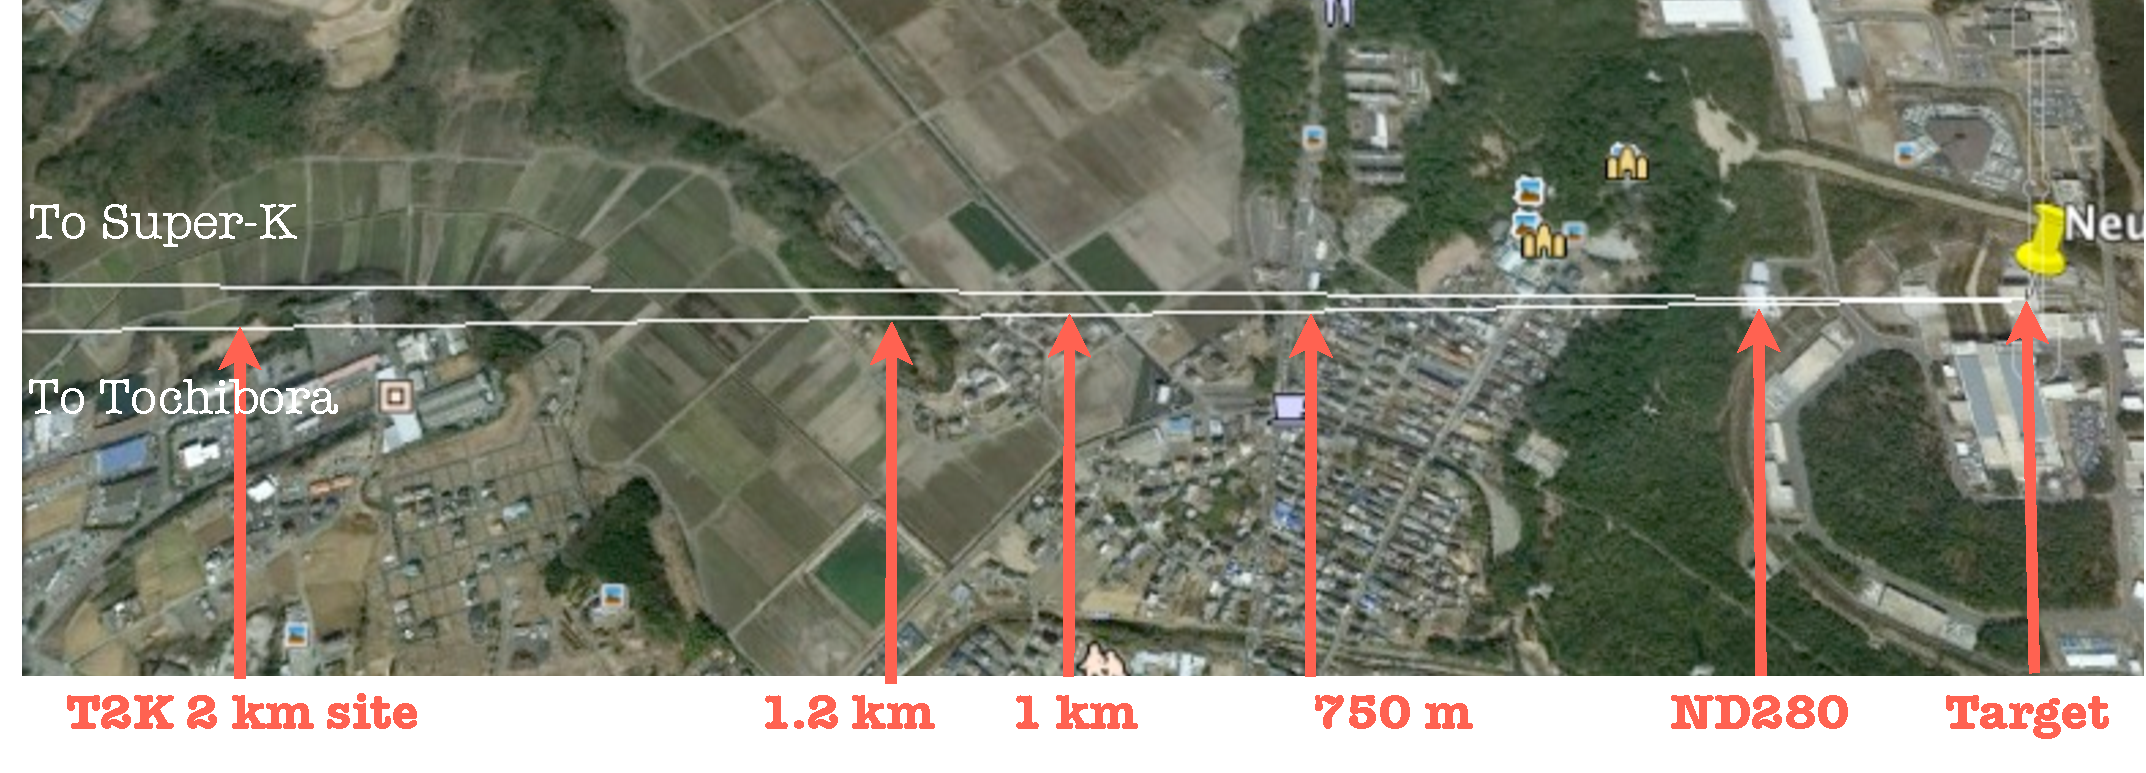
\includegraphics[width=15cm,angle=0]{figures/nuprismsites.pdf}
\caption{Potential sites are shown for \nuprism if all rice field locations are excluded.}
\label{fig:detsites}
\end{figure*}


The two far detector sites that must be considered are the Mozumi mine, where Super-K is located, and Tochibora, which is a candidate site for Hyper-K. There are four potential unused sites in the Tochibora and Mozumi directions, not including rice fields, a shown in Figure~\ref{fig:detsites}:
\begin{itemize}
\item 750m site near the Muramatsu community meeting centre:
          This location is right next to R245 and owned by the local government. The space is limited but covers the 
          Mozumi direction and the central line between Mozumi and Tochibora. This site would have the highest event pile-up rate.
\item 1km site: a large un-cultivated private land covering both Tochibora and Mozumi directions
\item 1.2km site: a large patch of private land at the foot of a forest covering both Tochibora and Mozumi directions
\item 1.8km site: the originally considered 2km detector site owned by the local government covering Tochibora direction. This site would have the deepest detector, 90m deep.
\end{itemize}
If the rice field can be available, there are a lot more choices. At the time of the 2km detector site study, rice fields were also considered, although not selected in the end. Changing the land use for the rice field would require additional approval process, if it were possible. 
The process of land use require consensus from the local community and the strong involvement of the host institution. There are facilities that are operated just outside J-PARC, the KEK-Tokai dormitory, KEK Tokai \#1 building at IQBRC, and  the dormitory of the Material Science Institute of Tokyo university about hundred meter north of IQBRC.
%\clearpage

\subsection{Civil Construction}\label{sec:civil}

%Section goals:
%\begin{itemize}
%\item Discussion of considerations from original 2km investigation \red{(TI)}
%\item Discussion of rock condition at various sites and implications for making a pit \red{(TI \& HKT)}
%\item Discussion of different pit construction methods with cost estimates \red{(AK \& HKT)}
%\end{itemize}

Based on the current baseline design of the \nuprism detector described previous sections,
we have communicated with companies for the preliminary cost estimation of
\nuprism civil construction; the water tank construction and detector construction.
The \nuprism detector is also considered as a prototype detector of Hyper-Kamiokande (Hyper-K) for
testing new photo-sensors, readout electronics, and the water containment system design.
%The detector parameters for the cost estimation are summarized as follows:
%\begin{itemize}
%% --------------------
%  \item Water tank
%    \begin{itemize}
%    \item A 10~m diameter and 50~m long deep cylindrical shape
%    \item Water containment system (e.g. tank lining, drain) is identical to Hyper-K
%    \end{itemize}
%% --------------------
%  \item Detector
%    \begin{itemize}
%    \item The detector 
%      consists of Inner Detector (ID) and Outer Detector (OD), and the detector moves
%      up and down for about 40~m in the water tank.
%    \item Positioning (elevating) accuracy of the detector assumes 10~cm or better, that
%      corresponds to 0.1~mrad or better accuracy of the off-axis beam angle
%    \item The detector moving speed assumes 40~m per 24 hours.
%% --------------------
%    \item Inner Detector
%      \begin{itemize}
%      \item 10~m high and 6~m diameter cylindrical shape (8~m diameter ID is also under consideration)
%      \item Uses 3000 of 8'' photo-sensors that provide about 40\% photo-coverage
%        (no photo-sensor housing)
%      \item ID is optically separated from OD by black sheet, like Super-K and Hyper-K
%      \item Use underwater readout electronics (Hyper-K prototype)
%      \end{itemize}
%% --------------------
%    \item Outer Detector
%      \begin{itemize}
%      \item 1.5~m thick active volume (0.5~m thick dead region between ID and OD)
%      \item Uses $\sim140$ of 20'' photo-sensors that provide about $\sim10$\% photo-coverage
%        with a housing (Hyper-K prototype)
%      \item OD surrounded by tyvek sheet, like Super-K and Hyper-K
%      \item Use underwater readout electronics (Hyper-K prototype)
%      \end{itemize}
%% --------------------
%    \end{itemize}
%\end{itemize}
%
%
%The cost estimation for the civil construction is divided into two parts;
%tank construction (excavation) and detector construction.


%% -------------------------------------------------
%\subsubsection{Candidate site \& geological information}
%% -------------------------------------------------
%
%\red{This subsection should be merged or replaced by Ishida-san's information}
%
%%\begin {figure}[h]
%%  \begin{center}
%%    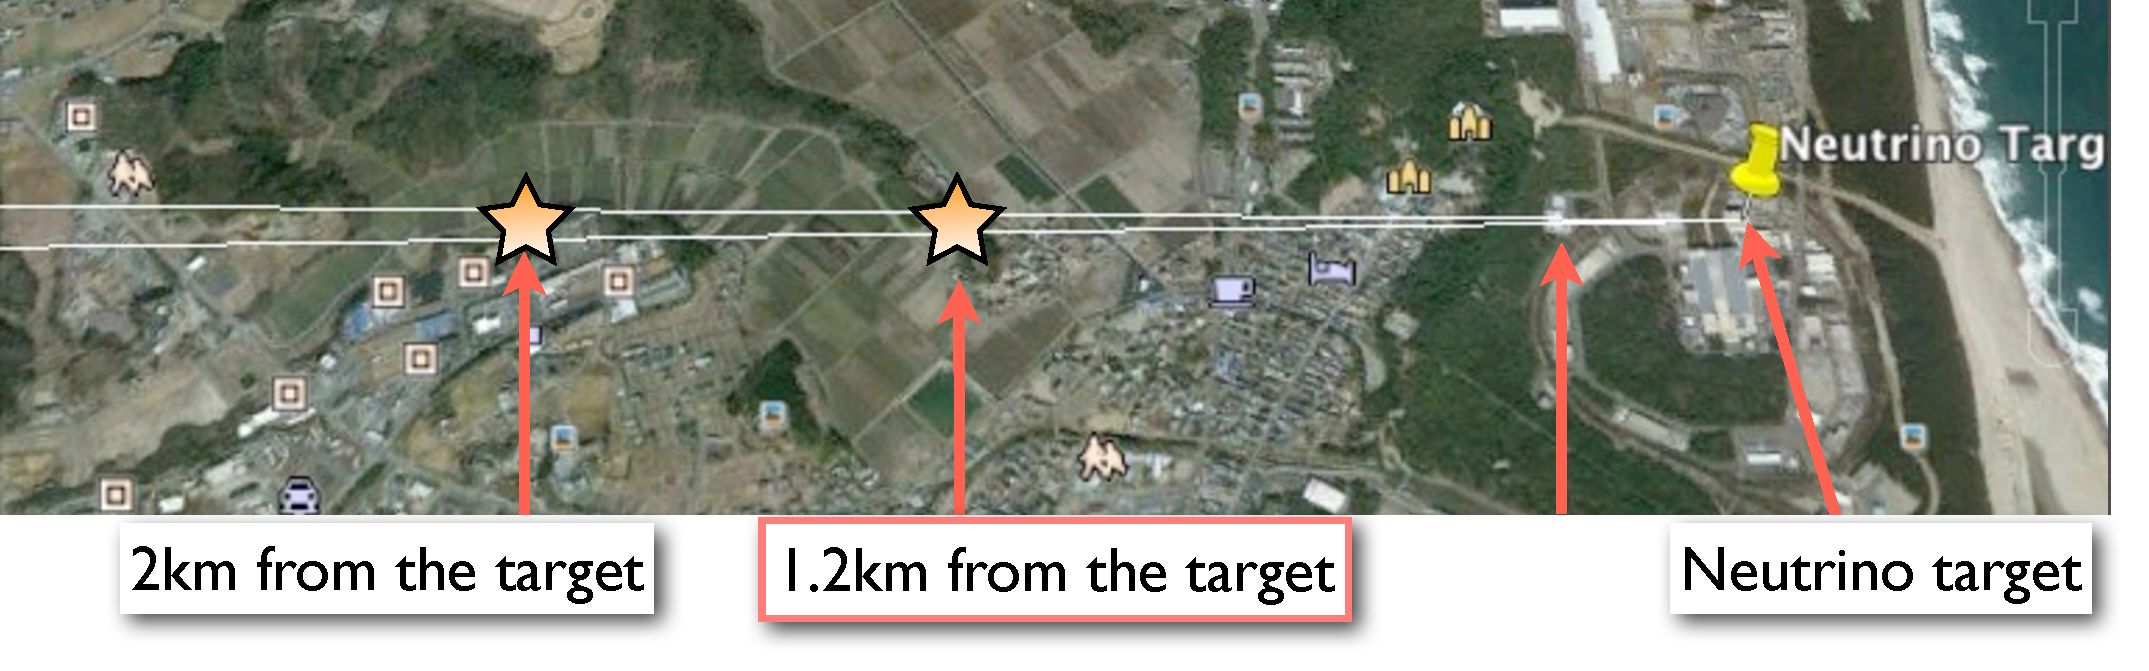
\includegraphics[width=0.7\textwidth]{figures/candidate_locations.pdf}
%%    \caption{Candidate locations for nuPRISM}
%%    \label{fig:candidate_location}
%%  \end{center}
%%\end {figure}
%%Figure~\ref{fig:candidate_location} shows candidate site locations.
%For the initial cost estimation, we assume ``1.2~km from the target'' is \nuprism detector site.
%Although there is no geological information at the exact location, several geological
%surveys have been carried out in the past at the candidate site vicinity (e.g. for public 
%construction works).
%Also, geological survey results at ``2~km'' are available.
%For the cost estimation, we estimate the geological condition at the 1.2~km site by extrapolating
%from the existing geological information.

% -------------------------------------------------
%\subsubsection{Excavation}
% -------------------------------------------------

Two groups have been contacted to provide preliminary cost estimates for the civil construction associated with fabricating a 50~m deep cylindrical volume with a 10~m diameter. The first group consists of a general construction company and a heavy industrial company currently providing cost estimates for Hyper-K. The second group is a single general construction company that was associated with the cost estimates from the original T2K 2~km detector proposal~\cite{t2k2km}.

There are several techniques to construct the 10~m$\phi$ and 50~m long vertical ``tunnel'';
Pneumatic Caisson (PC) method, Soil Mixing Wall (SMW) method, New Austrian Tunneling (NAT)
method, Urban Ring (UR) method.
Each of the construction methods have pros and cons, and some of the methods are not applicable
depending on the actual geological condition. Cost estimates from both construction groups are given in the appendix.

\subsection{Liner and Tank}

The \nuprism detector can be used for proof-testing various designs and components which
will be adopted in the Hyper-K detector. The \nuprism water tank will
have the same liner structure as that designed for Hyper-K.

The structure of the \nuprism tank liner is shown in Figure~\ref{fig:liner}. The innermost layer
contacting with the tank water must be a water-proofing component to seal the water within
the tank. We use High-Density Polyethylene (HDPE) sheets, which are commonly used as a
water-proofing tank liner material. The sheets have extremely low water permeability and also
are resistant to long-term damages from the ultra pure water. The adjoining sheets are
heat-welded, and the welded part also keeps the water-proof functionality.
%
\begin{figure}[htpb]
  \centering
  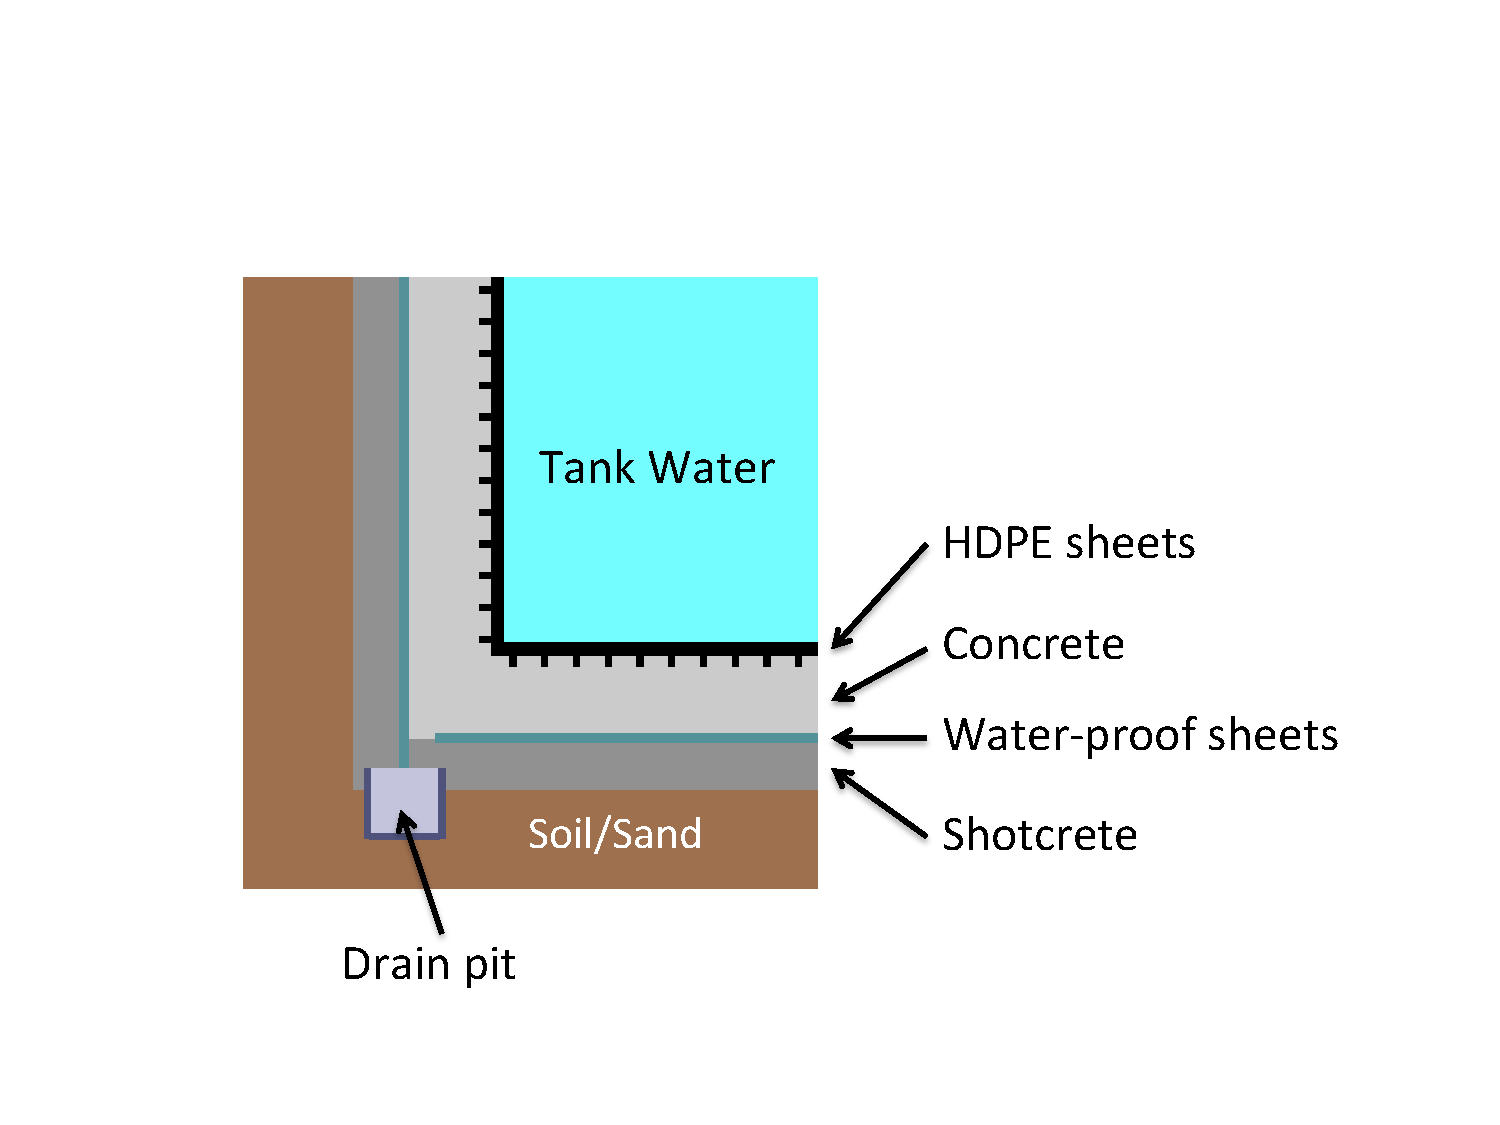
\includegraphics[width=0.5\textwidth]{figures/nuPRISM_liner}
  \caption{A schematic view of the \nuprism tank liner.}
  \label{fig:liner}
\end{figure}

We select the HDPE sheet with a number of studs protruding from one side. These studs work
for anchoring the sheet firmly on the backside concrete layer. To build this "HDPE on concrete"
liner, a HDPE sheet is fastened to the inside of a concrete form beforehand, then the concrete
is poured into the form for making the backfill concrete layer. While the thickness of the HDPE
liner is 5-10mm, the thickness of the backfill concrete layer is yet to be determined.

Though we aim to construct the HDPE sheet liner such that the tank water can not leak, an
additional water-proof layer is made between the backfill concrete layer and the shotcrete.
This layer works as a catcher and a guide for the water by the unexpected leakage through
the HDPE liner (and also the sump water through the shotcrete). This leaked water is drained
via pits placed under the water tank.

%The detailed information for the Hyper-K liner design (as a reference for the \nuprism liner)
%can be found elsewhere~\cite{hkmtg_tank_slides}.

\subsection{Detector Frame and Lifting Mechanism}

%Section goals:
%\begin{itemize}
%\item Describe PMT frame and rail system used to move the detector (RH talk from workshop)
%\end{itemize}


This section describes a proposed design for the frame that supports the \nuprism
PMTs and defines both the inner and outer detector.  We will also describe the system
by which this frame can be moved up and down in order to be able to make the \nuprism measurements.
Attention will be paid to the question of providing adequate water flow through the \nuprism
frame while maintaining optical separation.

\subsubsection{Detector Shape, Support and Positioning}
Figure~\ref{fig:detdesign} shows a simple cylindrical design, the walls of the Inner Detector (ID) 
being 0.5 meters thick. The half circles represent the 20'' PMTs (0.5m) facing outward for the veto
region (OD). The smaller half circles represent 8'' PMTs (0.2m) facing inwards to the ID region.
% Is this actually the right spacing for the ID or OD PMTs?  Seems to be too much space between them?
 The 0.5m thickness of the detector wall is to contain the bodies of the PMTs (and PMT electronis)
 and, with internal
 stiffening braces, be stiff enough to accurately position the PMTs and not deform significantly 
under the weights and buoyancies. 

Figure~\ref{fig:detdesign} also shows a conceptual support
 and positioning system. The detector is positioned on four vertical rails fixed to the shaft walls,
 and supported on top and bottom rings. Struts connect the detector to these two rings. The struts 
are positioned
 at the corners of the detector where the structure is strongest, and angled so that
 the distance from the detector to the start of the reflector is 1.7m top and bottom, and 1.5m
 on the sides. The reflector encloses the OD region and is required to be optically isolated from
 the ID volume, and from the shaft water volumes above and below. We discuss the reflector
 in more detail below.

\begin{figure}[htpb]
\centering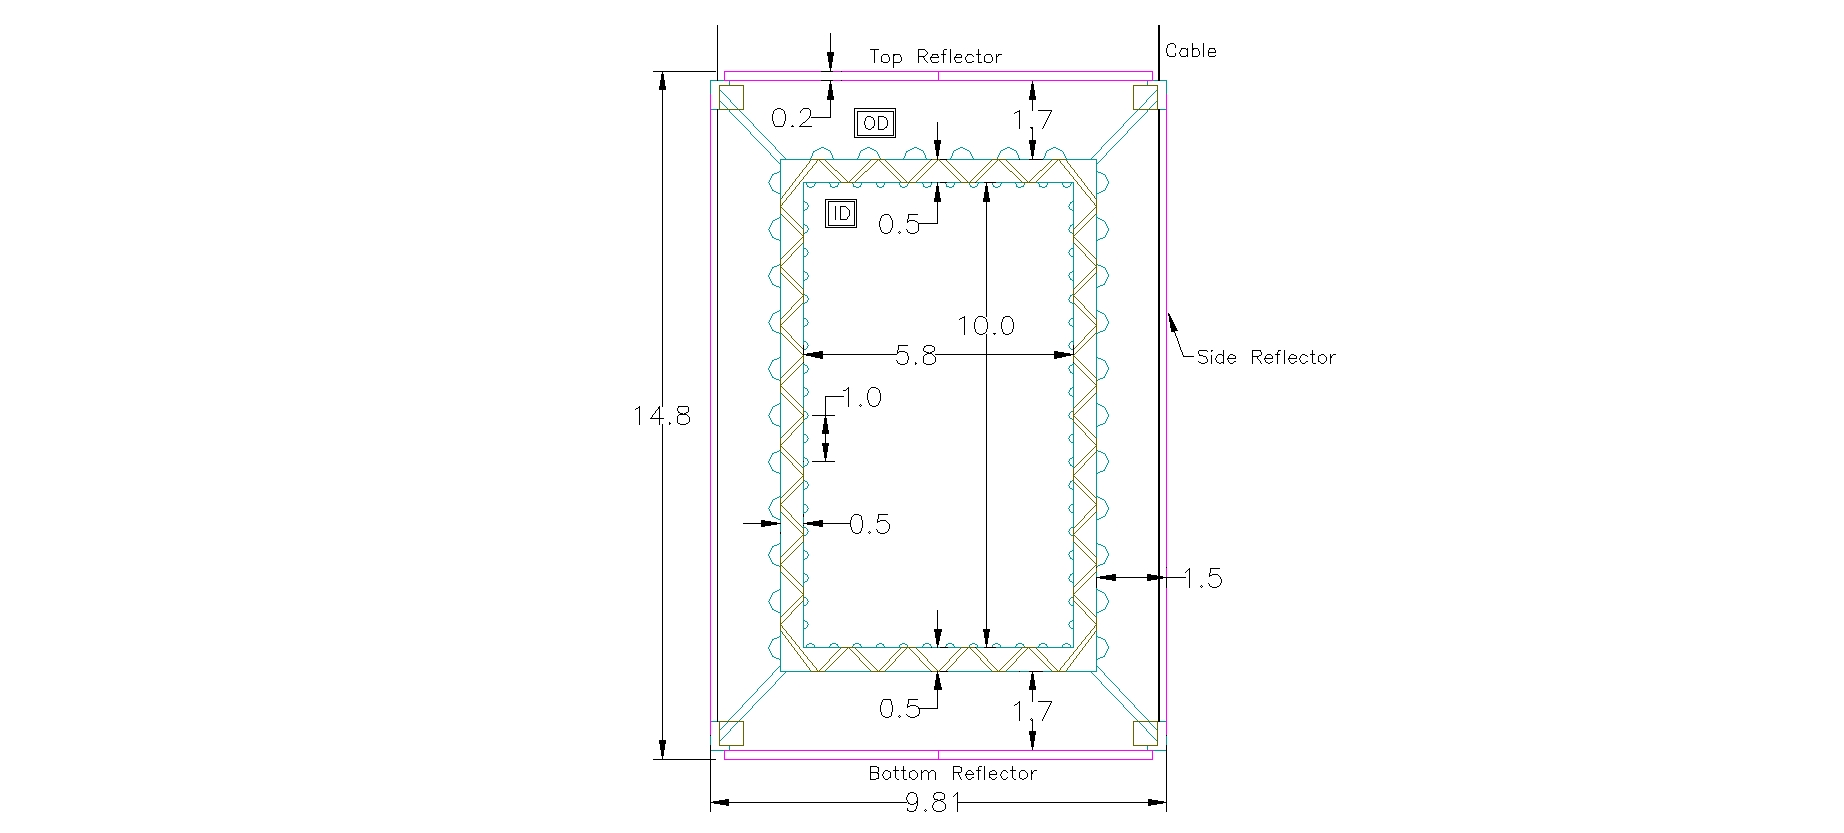
\includegraphics[bb=600 0 1450 820,clip,width=10cm]{figures/fig3-1.jpg}
\caption{The Detector is positioned on four rails inside shaft, and supported on top and bottom rings.
 Struts connect the detector to its rings. Four vertical cables support the assembly. Ballast can be 
added to the rings, if required. Distances are in meters.}
\label{fig:detdesign}
\end{figure}
% Might be nice to have a top view of the detector as well, to understand where struts rails go.

\subsubsection{Water Flow and Optical Isolations}

Figure~\ref{fig:detcomp} shows views of the top-left corner of the detector and reflector.
 Two section views indicate the conceptual features and functions involved. The volume of the ID and OD are $\approx$264m$^3$ and $\approx$790m$^3$, respectively, with a combined volume of $\approx$1,190m$^3$ 
(including all
 wall volumes). If the apparatus is to traverse the shaft limits in $\approx$24 hours, the speed
 would be $\approx$1.5 meters/hour. Since the reflector side walls are close to the shaft, the 
displaced water needs to flow through the reflectors. This speed corresponds to a water
 flow of $\approx$118 m$^3$/hour = 2.0 m$^3$/min. Even if the water could flow past the sides of the
 reflector enclosure, ~1,190 tons of water would also be in motion, which would be difficult to accommodate.
With no water flowing through the sides of the reflector enclosure, the sides can be
 simple metal panels with a white inner surface to enhance the OD light collection.
As indicated in Figure~\ref{fig:detcomp}, these vertical reflector walls need to 
notch around the four rails and the associated couplings on the rings, and would be screwed to the top/bottom rings. With a height of 13.8m
 and circumference of 33.5m, it will need to be segmented with overlapping joints
 (or added joint strips). When the detector is out of the water, it would be useful
 to be able to easily remove the side reflector segments. Minimal segmentation would
 be four, with joints at the center of the `notches'.
This would allow the segments  to slid out past the rails and the support towers.
The top and bottom reflectors
 are also bolted to the top/bottom rings, but they have to be thicker to allow them
 to be strong and stiff due to the quantity of water flowing through them. The stiffness is achieved by
 making the top/bottom reflectors 0.2m thick and them having an internal bracing
 structure.  The top/bottom reflectors need an optical seal to the rest of the
 shaft, yet allow $\approx$2.0 tons/min of water to flow through. Figure~\ref{fig:detcomp}, 
shows two possible solutions:


\begin{figure}[hptb]
\centering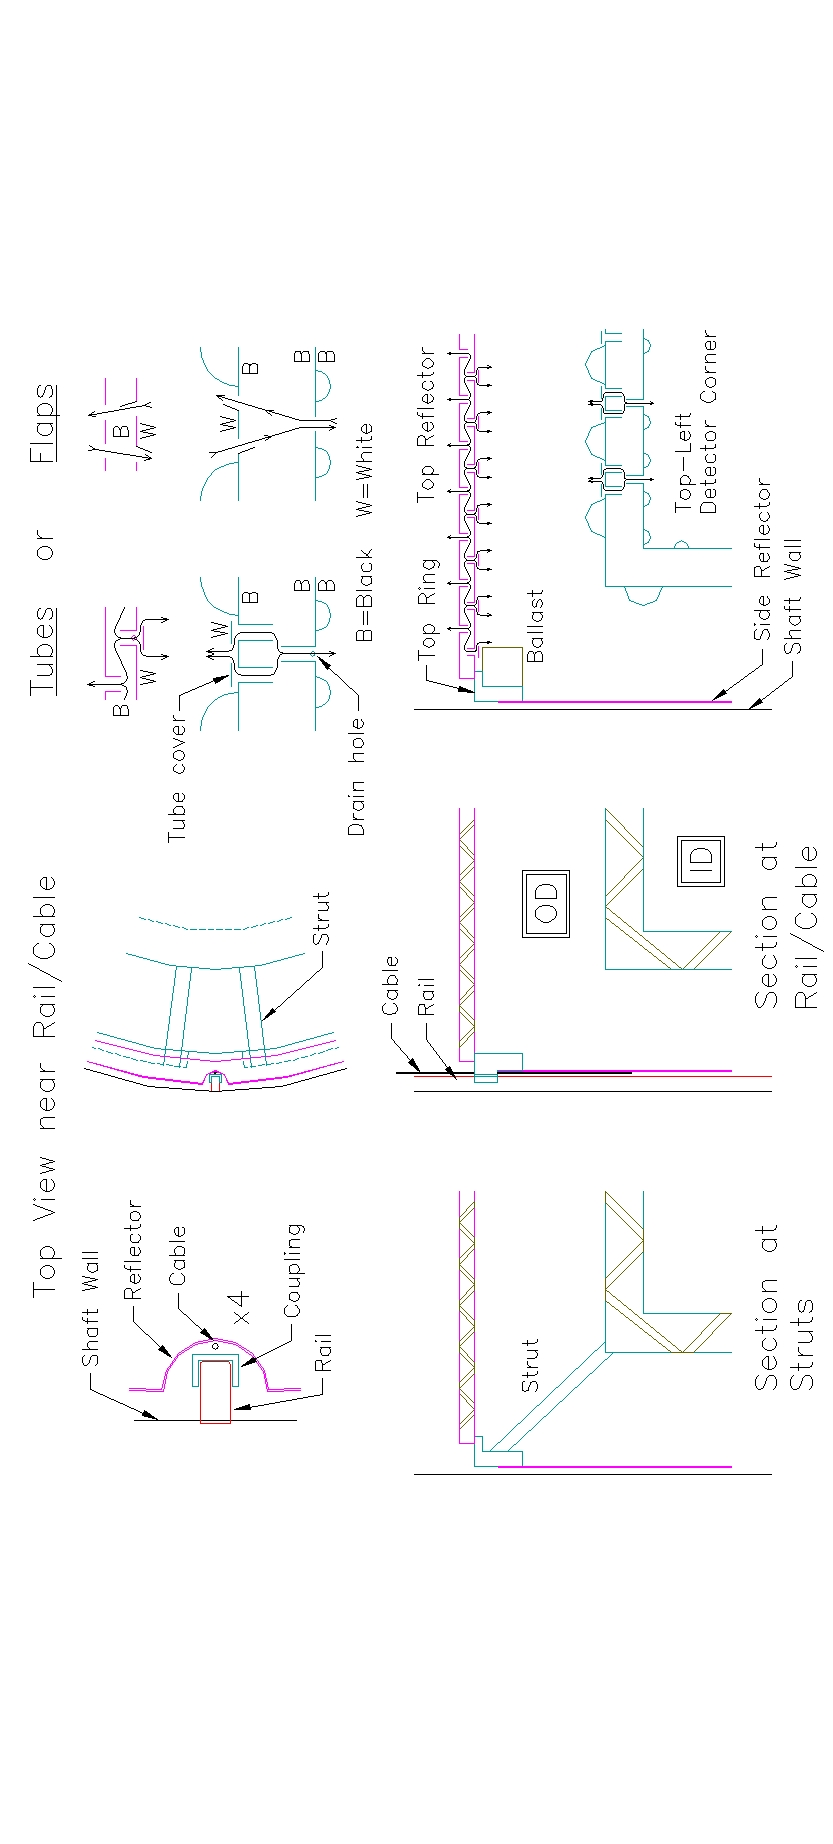
\includegraphics[bb=0 350 900 1750,clip,angle=270,width=10cm]{figures/fig3-2.jpg}
\caption{This shows views of the top-left corner of the detector and reflector. Two 
sections views indicate the conceptual features and functions involved. A system of
 offset black pipes (or flaps) would allow water to flow through.}
\label{fig:detcomp}
\end{figure}


\begin{enumerate}
\item The first is a system of offset black pipes, so that water can flow through,
 but any light would need at least two reflections off black surfaces. The inner
 surface of the top/bottom reflectors would be white to enhance light collection.
 The tubes at the inner surface would have white `tube covers'. This is easily
 done by having the tube extend, with the tube cover fixed to it, but the tube
 having four side large slots, leaving webs of material to hold the cover. The
 cover and outer surface of tube extension would be white. To prevent water
 being trapped in the reflector wall when the detector is lifted out of the
 water, there would be `Drain holes' in the tubes, just inside the inner wall.
 Alternately, there could be some small drain tubes+covers extending slightly into OD
 volume. This scheme is a little complicated, but has the advantage of no moving parts. 
If the flow is fully distributed over the 55.0 m$^2$ area, the movement water flow would
 then be $\approx$36 liters/minute/m$^2$.
 
\item Another way solve this
 problem would to have a system of flaps that open only when the detector is moved,
 and close automatically when it stops. Half the flaps open when the detector moves
 down (water moves up), these flaps close under their own weight when movement stops.
 The other flaps open when the detector moves up (water down), these `down' flaps
 would need to be spring loaded or counterweighted to close when movement stops.
 In Figure~\ref{fig:detcomp}, we show both these flaps in the open position. The inner surfaces
 of the flaps would be white. In this scheme most of the water would drain through the spring
 loaded `down flaps', but would also require a system to small holes or pipes to drain out
 the last of the water. This system has many moving parts that cannot be lubricated, so
 binding and galling would be concerns, but it can probably be made to work. It would
 need to be made very reliable, a few flaps stuck closed wouldn't be a concern, but some
 stuck open could be a problem. This system has the disadvantage that it prevents lower
 levels of circulating water during data taking. This recirculating loop will probably
 be required for; the purification and temperature control of the water, cooling of
 electronics etc. For these reasons, we prefer the offset tubes option.
 % I think that clearly recirculating will be needed, so this is a little oddly phrased.

\end{enumerate}


When the detector is out of the water, the bottom reflector would need to be segmented to
 be removed between the support towers. With four towers (see Figure~\ref{fig:dettower}),
 the four bottom cover segments would be 4.6x4.6 meters. Higher segmentation (multiples of
 4) would also be possible. We imagine a scissor cart rolled under the detector, lifted to
 contact a segment. It could then be unbolted, lowered and rolled away. The segments would
 need to overlap on the inner surface for light seal, and on the outer surface for joining
 (or have extra joint strips). The top reflector would be craned out, in one piece or in
 segments.




\subsubsection{Walls of Inner Detector (ID)}
The top/bottom walls of the
 ID would also need to allow water flow, otherwise one would have to allow for
 the inertia of 400 tons of trapped water. The movement flows would be 42 tons/hour =
 0.7 tons/minute. Distributed, this is 27 liters/minute/m$^2$. This is somewhat less than
 the 36 liters/minute/m$^2$ of the reflector, but this wall has all the PMTs as well. In
 Figure~\ref{fig:detcomp}, I show the tubes and flaps options for this wall, similar
 to that for the top and bottom reflectors.

\subsubsection{Detector in the shaft}

The detector is guided within the shaft by a set of rails.
The current proposal has
 four rails and support cables but it could be three, five, etc. if dictated by other design considerations.
 It is important to understand that the ring connections to the rails do not need to be
 high precision rail bearings. Because the positioning accuracy required is only $\approx$1cm,
 they could be simple guides (see Figure~\ref{fig:dettower}). Similarly, the rails do not need to be
 complex. The loose tolerance makes it far less likely that the detector will jam on
 the rails. When the detector has been moved, there may be a system to lock two of the
 four guide locations to eliminate small position changes during data taking. Another
 reason for a looser coupling (before locking), is that then the rails do not need to
 be so precisely positioned on the shaft walls, i.e. several  millimeters versus
 0.1mm. 

Figure~\ref{fig:dettower} shows the detector in the shaft, the shaft covers
 and the external towers. Four vertical cables support the assembly. Ballast can be
 added to the rings, if required. Above ground, there would be four towers extending
 upwards ~17.6 meters. Four motors, acting together, lift or lower the detector in
 the shaft, or even lift it completely out of the water. The load will increase as
 it leaves the water (loss of buoyancy), if the load is too much, the top ballast
 can be removed by crane as it clears the water. Or, a lifting frame could be attached
 when the top ring clears the water, allowing the crane to raise it further, then it can
 be locked in the out position, freeing the crane.

In this concept, the signal and
 power cables for the detector would travel up out of the water beside the four support cables.
 They would nominally go up and over the towers, then down to the ground racks. With this
 scheme there would be no extra length in the water, wherever the detector was positioned
 in the shaft. When the detector is slowly lowered further down the shaft, the cables etc.
 should be cleaned before entering the water.


\begin{figure}[htpb]
\centering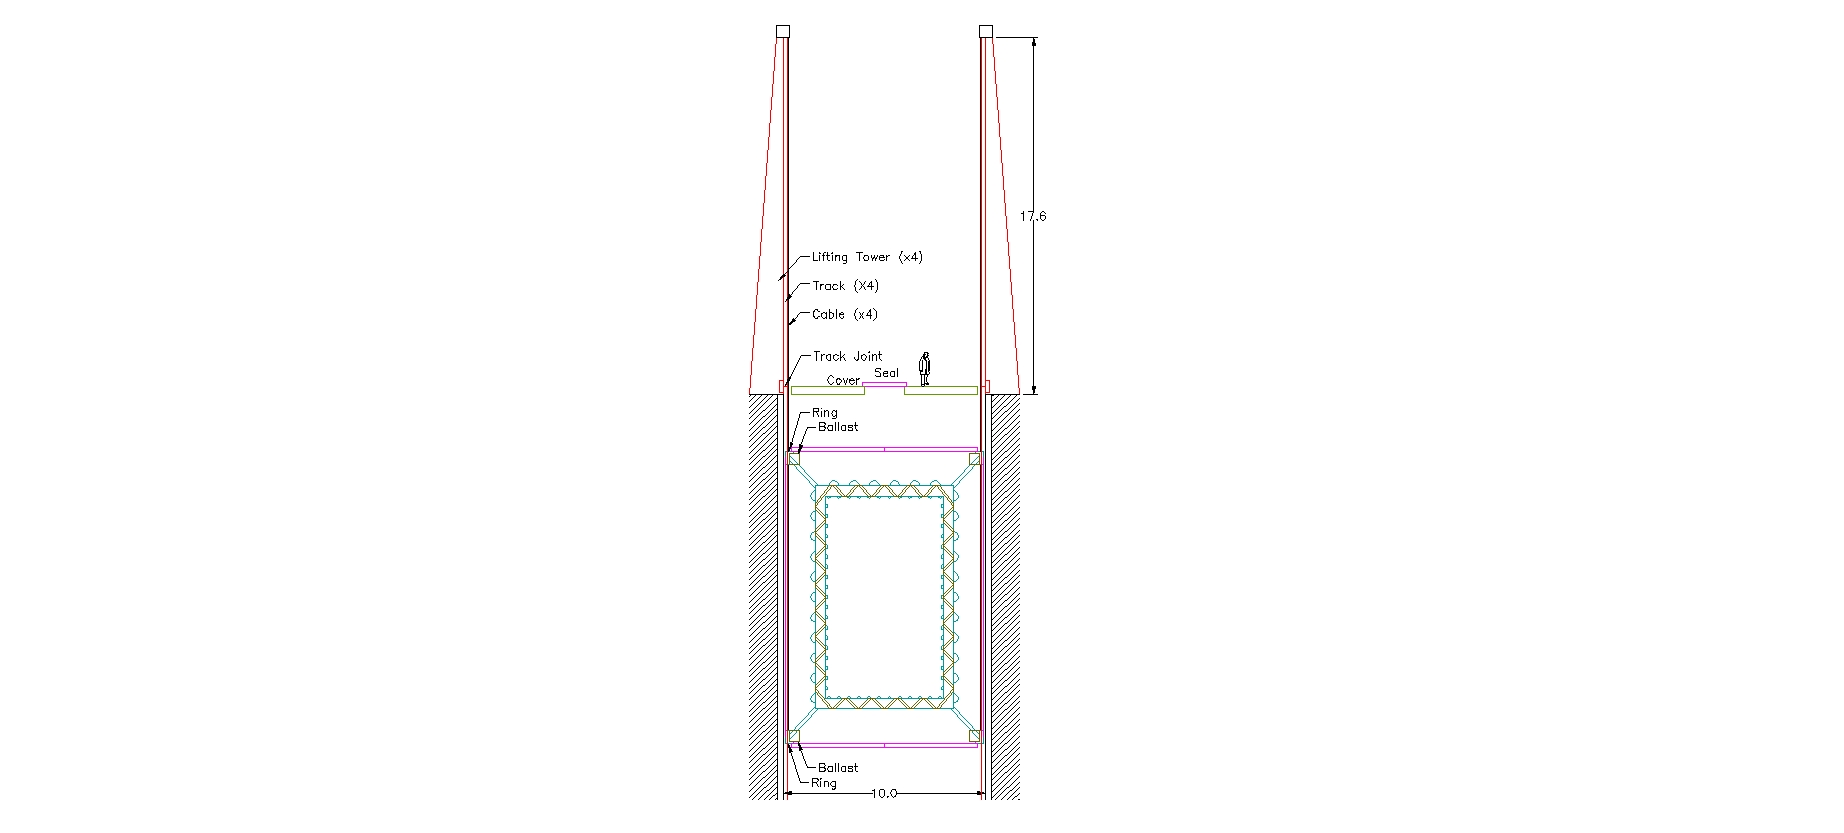
\includegraphics[bb=750 0 1050 850,clip,width=7cm]{figures/fig3-3.jpg}
\caption{This shows the detector in the shaft, the shaft covers and the external towers.
 Four vertical cables support the assembly. Above ground, there would be four towers upwards
 extending 17.6 meters. Four motors, acting together, lift or lower the detector in the shaft,
 or even lift it completely out of the water.}
\label{fig:dettower}
\end{figure}

Once the detector is entirely out of the water, the shaft covers can be craned back into
 position (see Figure~\ref{fig:detcover}). Adding counterweights will 
make sure the Center-of-Gravity (COG)
 of the covers are beyond the detector shadow when the covers are pushed in. 
The covers would be bolted to the ground.
 Lightweight seals cover the joints, the central region, and the four small areas where the support
 cables, signal and power cables exit the water.

\begin{figure}[htpb]
\centering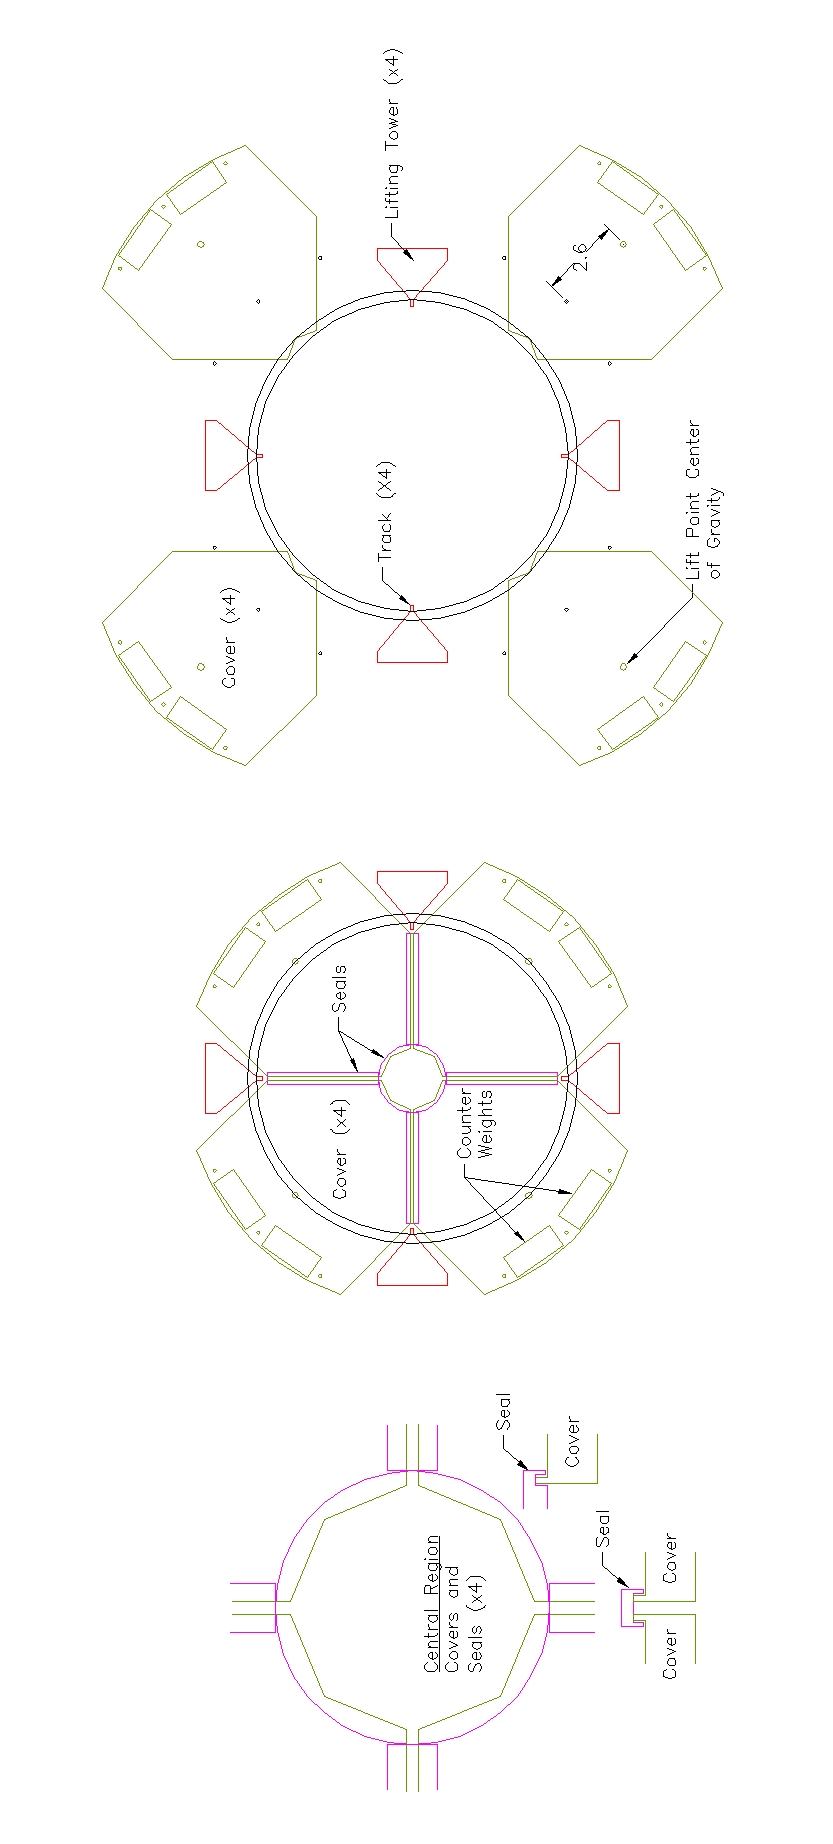
\includegraphics[bb=0 0 800 1000,clip,width=7cm,angle=270]{figures/fig3-4.jpg}
\centering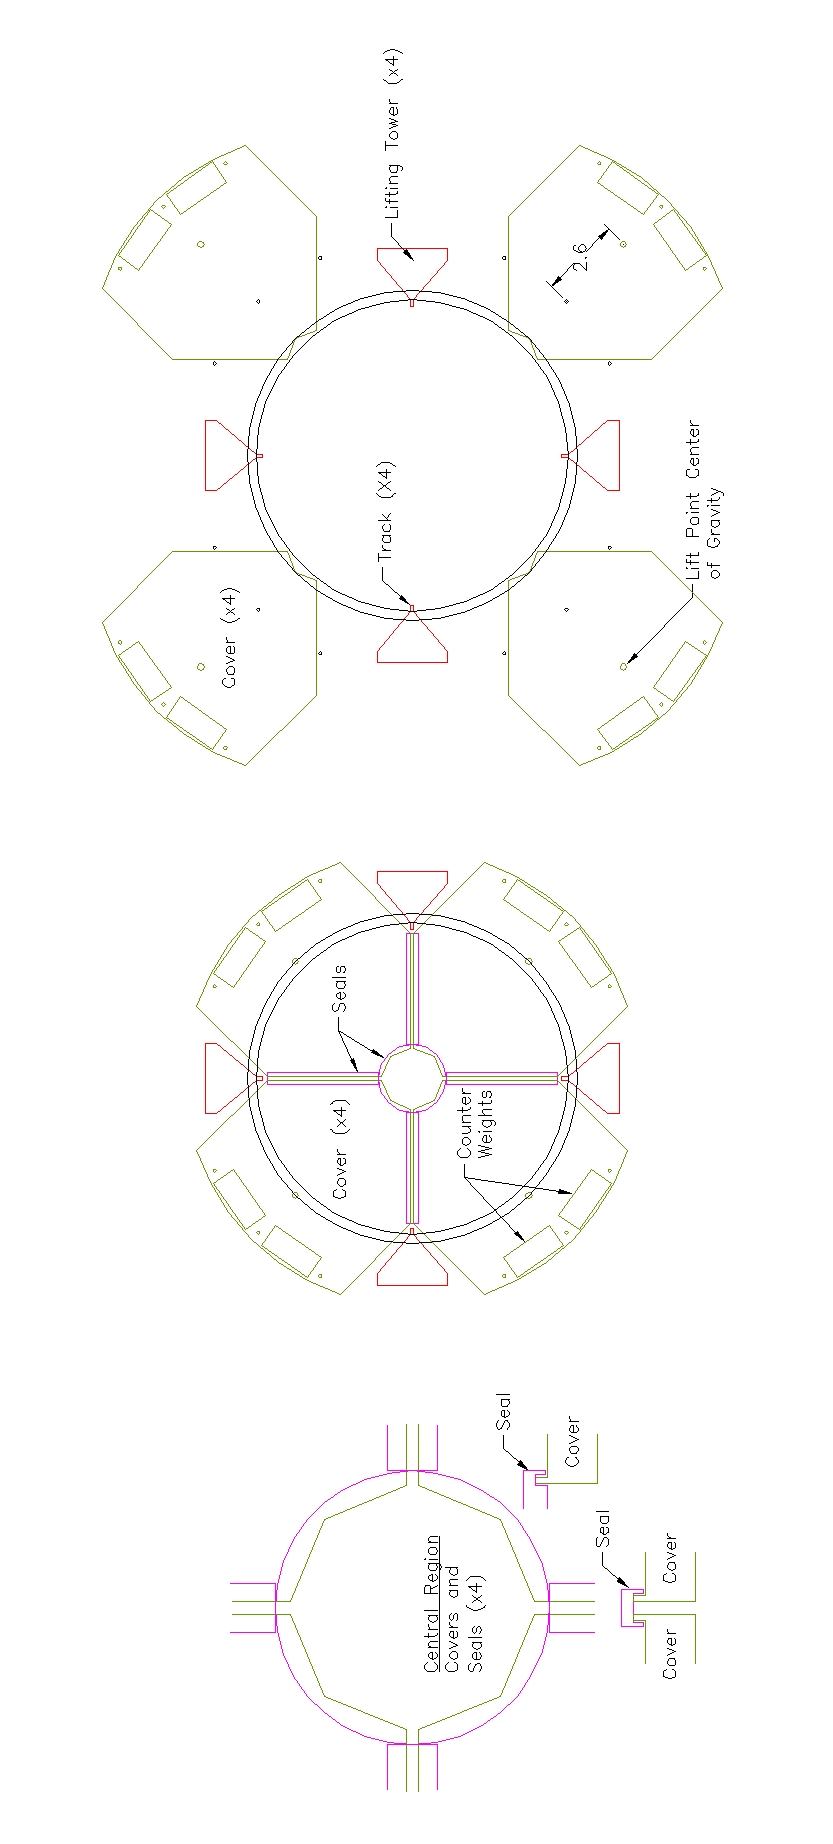
\includegraphics[bb=0 1000 800 1800,clip,width=7cm,angle=270]{figures/fig3-4.jpg}
\caption{The four covers can be craned in and out. Added counterweights make sure the center of
 gravity is beyond the detector shadow when in. The covers are bolted to the ground. Light weight seals
 cover the joints and the central region.}
\label{fig:detcover}
\end{figure}

Figure~\ref{fig:detremoved} shows the detector out of the water and covers reinstalled. It is important that
 the covers and seals are safe for people and light equipment, so that the bottom of the detector can be
 worked on. Scaffolding can be erected to work on all parts of the detector. The figure also shows the
 detector moved to a stand. To move the detector, the lifting frame would be installed, the detector
 supported, then the eight ring guides removed and two of the towers removed (or laid down), opening
 a path for the detector move.

Whether above the shaft or on a separate stand, it would probably
 be useful to be able to remove the reflector sections and get access to parts of the ID.
 If the ID were bolted together sections, it might be possible to partially disassemble to make repairs and/or replacements.

\begin{figure}[htpb]
\centering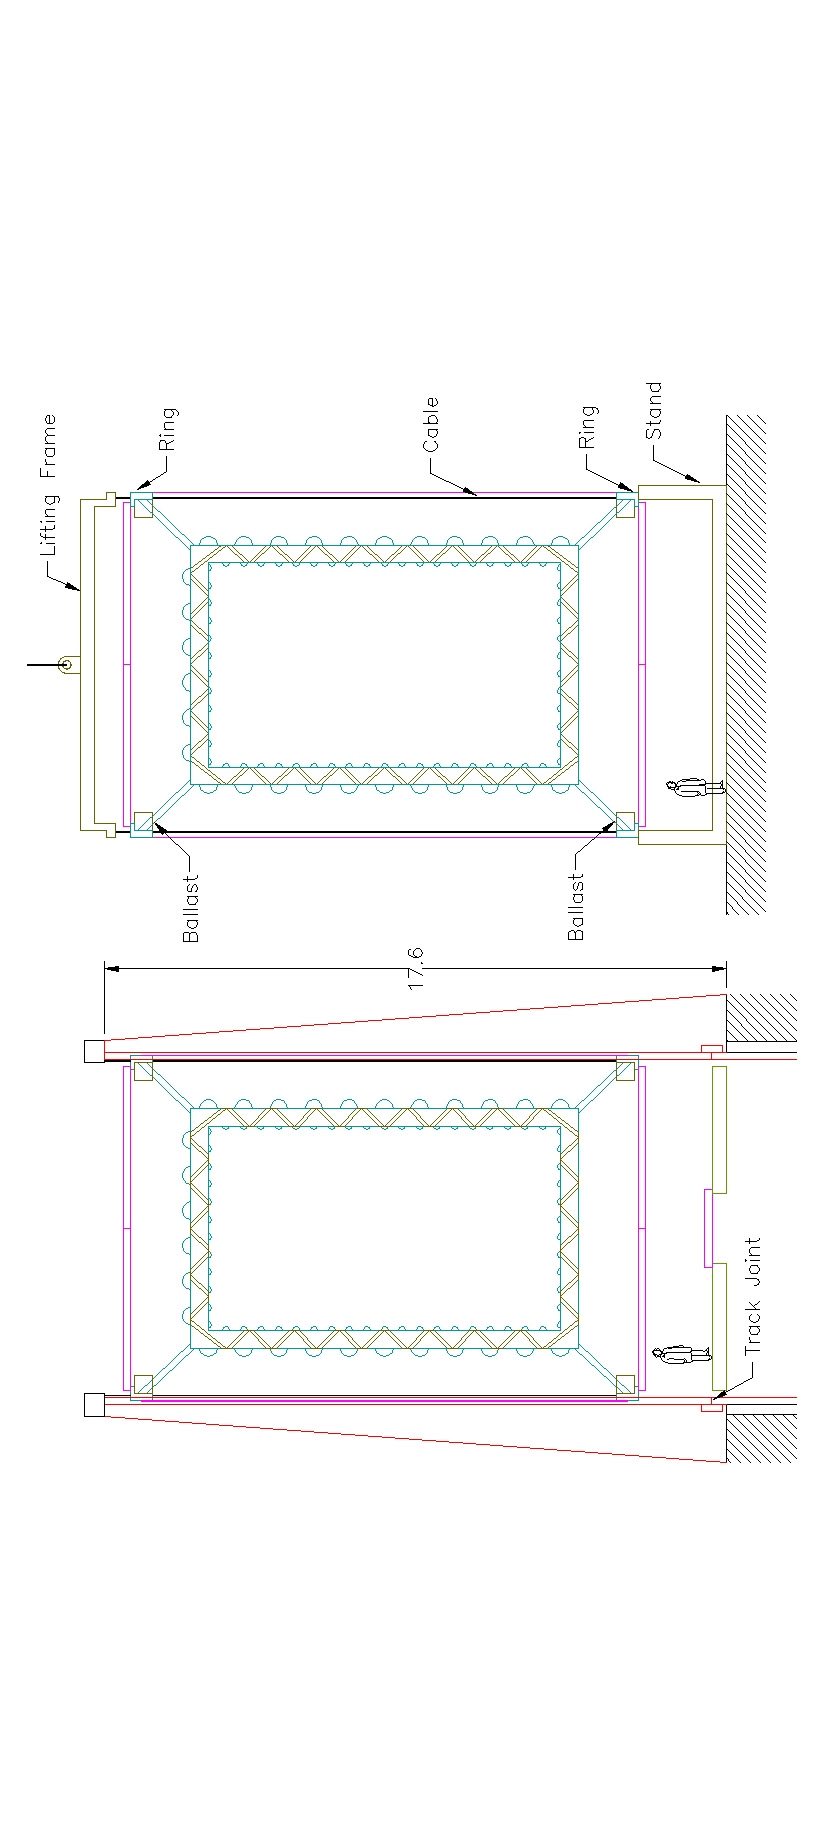
\includegraphics[bb=0 300 800 900,clip=true,width=10cm,angle=270]{figures/fig3-5.jpg}
\caption{The four towers allow the detector to be raised out of the water (units in meters). The covers  can be reinstalled under the detector, allowing people to work underneath it. A lifting frame can be craned over the detector, attached, and the towers removed. The detector can then be craned to a stand.}
\label{fig:detremoved}
\end{figure}


\subsubsection{Detector Surveying}

As mentioned earlier, after the detector has been moved,
 there may be a system to lock two of the four guide locations to eliminate small position
 changes during data taking. A laser surveying system could be in place to look down through the
 water to periodically check the detector position at the four rail locations. The PMTs may have
 to be turned off during these times. The positioning of PMTs within the detector would be surveyed
 during its assembly (out of water) and then should only be subject to thermal expansion/contraction
 shifts in the water, plus deflections due to loads (primarily the top/bottom PMTs.

The thermal
 expansion/contractions of the detector will depend on its material. For a 10 meter Aluminum piece,
 the expansion would be ~2.2mm for a 10 OC change. 306 stainless steel would be ~1.6mm. The shaft, being reinforced concrete, should expand ~1.3mm for 10 degrees. Stainless steel is
 a better thermal match, the differential expansion being ~0.3mm for 10 degrees, compared to ~0.9mm 
for an Aluminum detector frame, but the difference is not likely to be significant.

%\afterpage{\clearpage}

\subsection{Scintillator panels}\label{sec:scint}

The veto system of the \nuprism detector can be composed of plastic scintillator detectors which completely surround the the water Cherenkov detector. The main purpose of the veto system is to identify backgrounds from beam neutrino interactions in the surrounding pit walls  and to provide a cosmic trigger signal for calibration purposes. The technology developed for the ND280 SMRD detector can be applied for this veto system.

\subsubsection{Scintillator counters with WLS/avalanche photodiode readout}

Scintillator counters with wavelength-shifting (WLS) fibers and opto-electronic readout are an established technology for neutrino detectors in  long-baseline neutrino oscillation experiments. ND280 consists of several subdetectors which use extruded plastic scintillators of various shape and dimensions~\cite{nd280}. Each of these subdetectors is comprised of plastic slabs and bars, wavelength shifting fibers and compact photosensors - multi-pixel avalanche photodiodes. The Kuraray  double-clad Y11 WLS fibers are used in all ND280 scintillator detectors for transportation of the reemitted light to photosensors.  

%{\it Photosensor}. Multi-pixel avalanche photodiodes operating in a limited Geiger mode are used as photosensors in the ND280. Such devices consist of many independent sensitive pixels each of which  operates as an independent Geiger micro-counter with a gain of the same order as a vacuum photomultiplier tube. Geiger discharge is initiated by a  photoelectron in a high electric field locally created by  the applied  bias voltage in a very thin  layer ($\sim$1~$\mu$m p-n junction).   Detailed information   and basic principles of operation of multi-pixel  photodiodes can be found  in a  review  paper~\cite{renker} and references therein. The first  application of such devices in a real long-term experiment is done in the T2K experiment which uses about 56000 of  the customized 667-pixel Hamamatsu Multi Pixel Photon Counters (MPPC) S10362-13-050C with sensitive area of $1.3\times 1.3$ mm$^2$~\cite{mppcT2K} in the ND280. 
  

%The main parameters of MPPC (gain, photon detection efficiency, intrinsic noise, cross--talk, after pulses) depend on the applied bias voltage, $V_{bias}$, or, more accurately, on $\Delta V = V_{bias} - V_{bd} $, where $V_{bd}$ is the breakdown voltage of the photodiode.
%The photodiode gain is determined by the charge accumulated in a pixel capacitance $C_{pixel}$: $Q_{pixel} = C_{pixel}\cdot\Delta V$,  where the overvoltage $\Delta V$ is  a difference between the applied voltage and the breakdown voltage of the photodiode. For MPPC's have the operation voltage of about 70 V and  a gain in the range  $(0.5 - 1.5)\times  10^6$. When a photoelectron is produced it creates a Geiger avalanche.   The amplitude of a single pixel signal does not depend on the number of carriers created in this pixel. Thus, the photodiode signal is a sum of  fired pixels.
%Each pixel operates as a binary device, but the multi--pixel photodiode as a  whole unit is  an analogue detector with a dynamic range limited by the finite number of  pixels.  

%The  photon detection efficiency (PDE) of a multi-pixel  avalanche  photodiode 
%is a product of 3  factors:
%\begin{equation}
%{\rm PDE} = QE\cdot\varepsilon_{Geiger}\cdot\varepsilon_{pixel},
%\label{eq:pde}
%\end{equation}
% where $QE$ is the wavelength dependent quantum efficiency,  
% $\varepsilon_{Geiger}$ is the probability  to initiate the Geiger discharge 
% by a photoelectron, and $\varepsilon_{pixel}$ is a fraction of the total 
% photodiode  area occupied by sensitive pixels. The  bias voltage affects 
%one parameter  in expression~(\ref{eq:pde}),  $\varepsilon_{Geiger}$.   
%The geometrical factor $\varepsilon_{pixel}$  is  completely 
%determined by the photodiode topology, and is in the range 50-70\%.    The   
%PDE of a $1.3\times 1.3$ MPPC used in ND280  as function of wavelength of detected light is shown in 
%Fig~\ref{fig:pde_mppc}.
%\begin{figure}[h!]
%\centering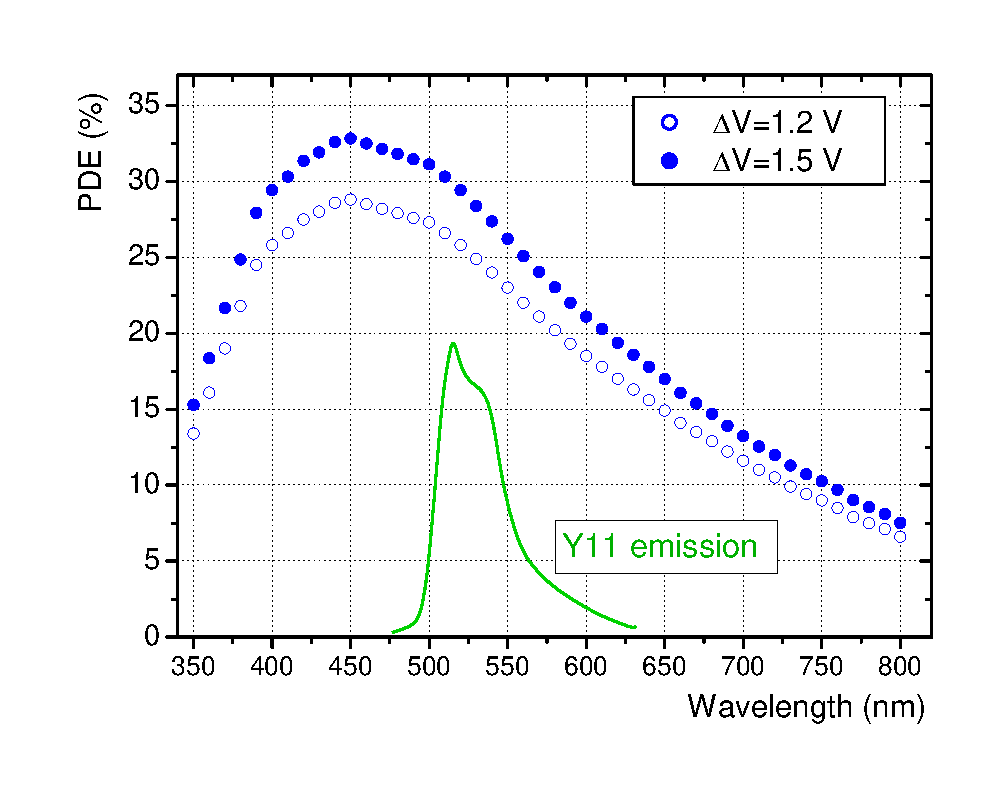
\includegraphics[width=10cm,angle=0]{figures/Y11_MPPC.eps}
%\caption{Photon detection efficiency  of an MPPC as a function of wavelength of the detected light at  $\Delta V$ of 1.2 and 1.5~V at 25$^{\circ}$C. 
%The Y11(150) Kuraray fiber emission spectrum (in a. u.) for fiber length of 150 cm (from Kuraray spec) is also shown.}
%\label{fig:pde_mppc}
%\end{figure}
%
%The PDE of new Hamamatsu devices developed over last 2-3 years was significantly increased. For example, the PDE of MPPC S12651-050C with 50$\mu$m cells is about 50\% for wavelength of 400-550 nm, as seen in Fig.~\ref{fig:pde_new_mppc}. 
%\begin{figure}[h!]
%\centering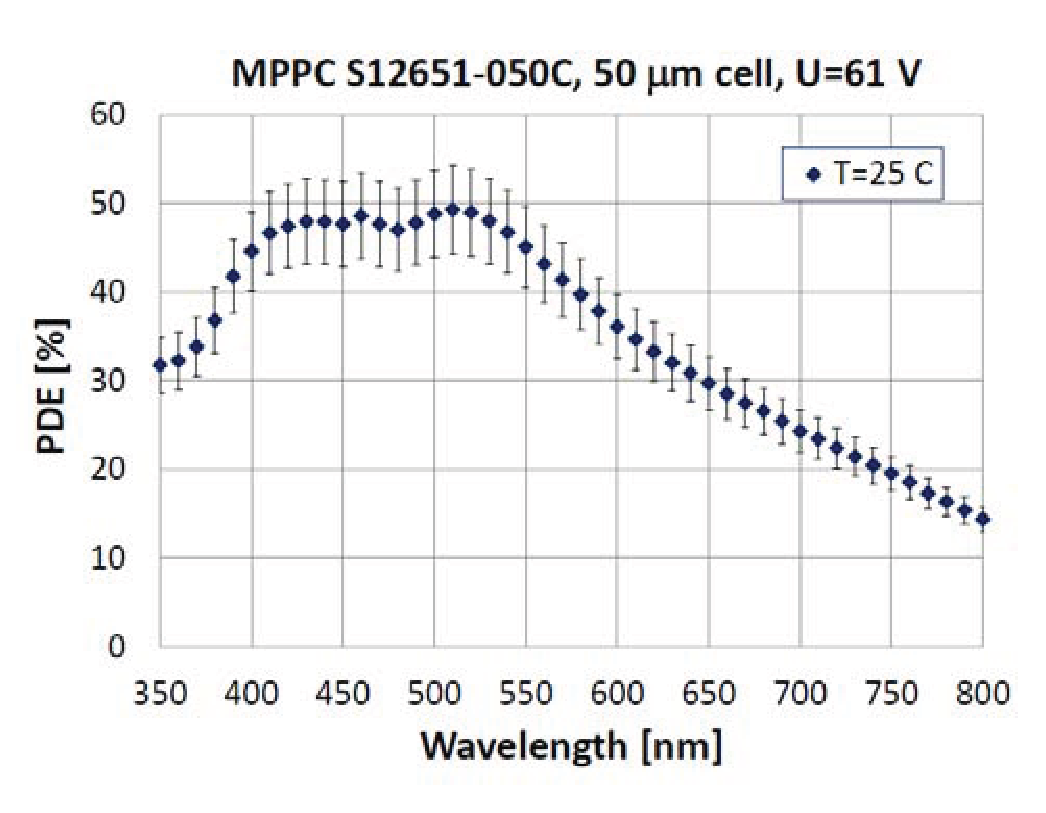
\includegraphics[width=10cm,angle=0]{figures/pde_new_mppc.eps}
%\caption{Photon detection efficiency  of the MPPC S12651-050C as a function of wavelength of the detected light~\cite{musienko_instr14}.}
%\label{fig:pde_new_mppc}
%\end{figure}
%
%It should be also noted that cross-talk and after pulses were greatly reduced in new MPPC devices. Moreover, the gain of new MPPC's have rather small temperature dependence  due to higher operational overvoltage. 
 
{\it SMRD counter}. The SMRD detector was made of the polystyrene-based scintillator slabs, each with an embedded wave-length shifting  fiber. The slabs were produced at the Uniplast Factory (Vladimir, Russia). The scintillator composition is a polystyrene doped with 1.5\% of paraterphenyl (PTP) and 0.01\% of POPOP. The slabs were covered by a chemical reflector by etching the scintillator surface  in a chemical agent that results in the formation of a white micropore deposit over a polystyrene\cite{extrusion}.  The chemical coating is an excellent reflector, besides it dissolves  rough surface acquired during the cutting process. The WLS fiber was read out on both ends to increase light yield, improve uniformity and position accuracy, and provide redundancy.
%(see Fig.\ref{fig:smrd_slab}).
%\begin{figure}[h!]
%\centering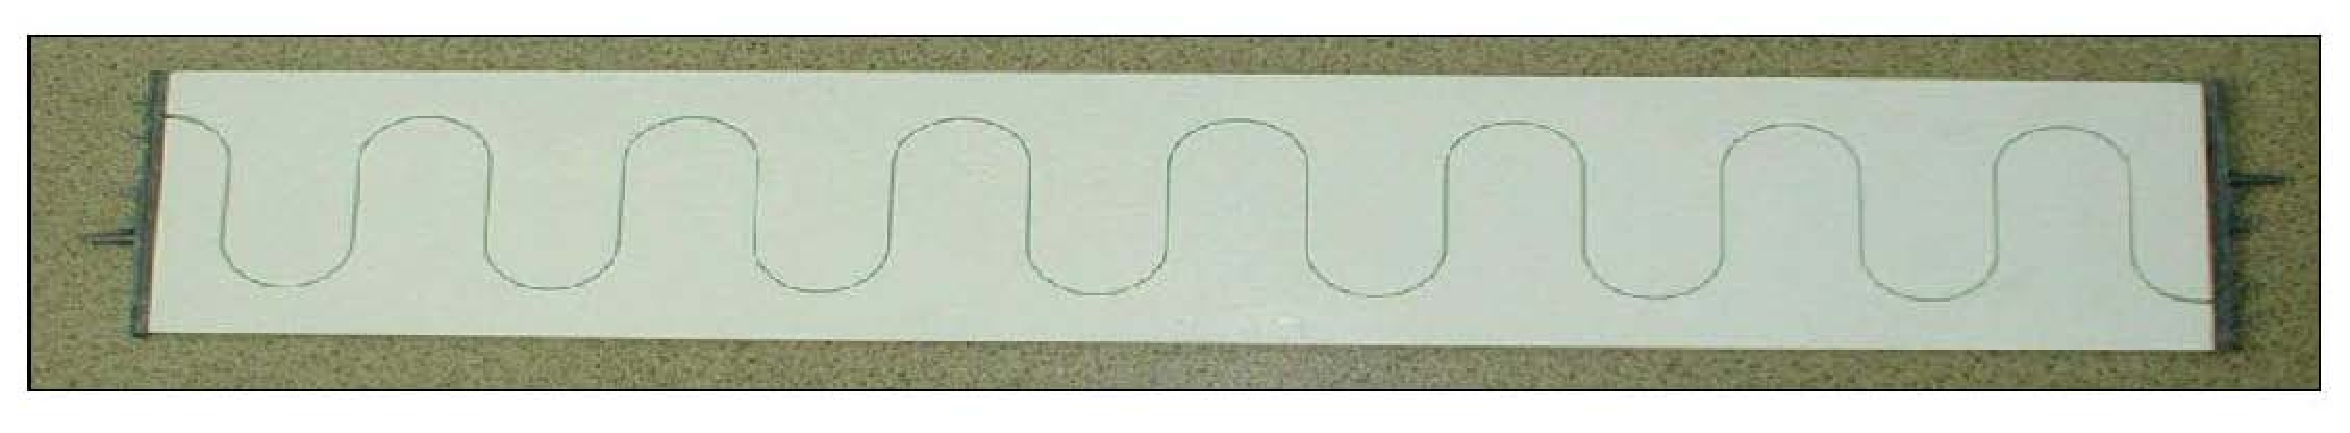
\includegraphics[width=14cm,angle=0]{figures/slab.eps}
%\caption{SMRD scintillator slabs with a serpentine-routed Y11 WLS fiber.}
%\label{fig:smrd_slab} 
%\end{figure}

A key feature of   these counters is the usage of the one serpentine-shaped WLS fiber for readout of scintillating signal.   The serpentine geometry of a groove consists of 15 half-circles, each with a diameter of 58 mm and straight sections connecting the semi-circles. A 1 mm diameter Y11 (150) Kuraray WLS fibers of flexible S-type and with double-cladding was used for the SMRD counters. Fibers are bent into a serpentine-shape and glued into grooves with BC600 Bicron glue.
%The light yield distribution  of all SMRD counters is shown in Fig~\ref{fig:smrd_ly}.
%\begin{figure}[h!]
%\centering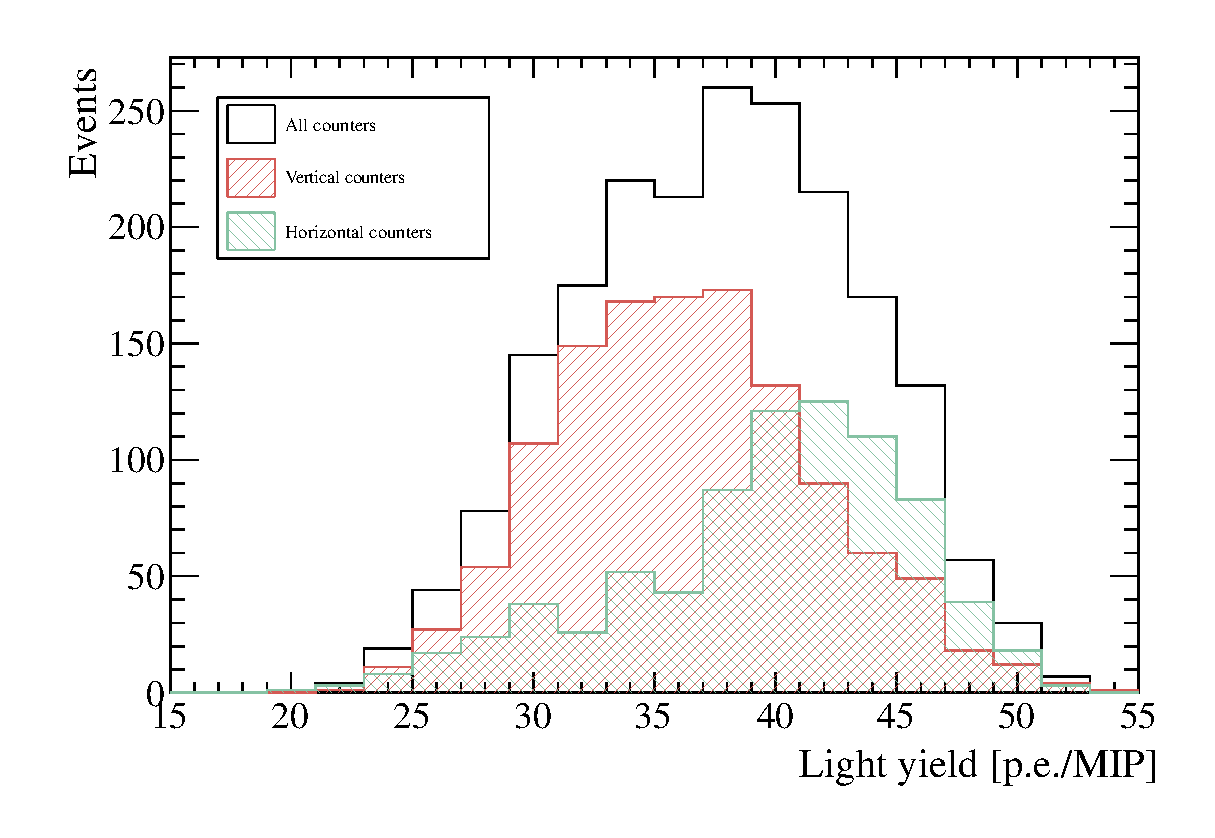
\includegraphics[width=12cm,angle=0]{figures/smrd_ly.eps}
%\caption{The light yield (sum of both ends) distribution for 2024 SMRD 
%counters.}
%\label{fig:smrd_ly}
%\end{figure}
%As seen from this figure, 
The mean light yield for sum of both ends  was about 40 p.e./MIP after subtraction of the MPPC cross-talk and after pulses. The high light yield allowed us to obtain the efficiency of more than 99.9\% for detection of  minimum ionizing particles.

%{\it Long fibers}. To test the performance of scintillator detectors with longer WLS fibers,  
%90~cm long and 0.7~cm thick scintillator slabs were extruded.   
%A 2~mm deep and 1.1~mm wide groove was machined along a bar central line to accommodate the 16~m long Y11 fiber. Since a tested bar is moved along the fiber the optical coupling between the fiber and the bar was implemented with an optical grease.
%Tests of scitillator bars  with embedded WLS fibers and MPPC's showed very good results, as seen in Fig.~\ref{fig:bar2}.
%\begin{figure}[h!]
%\centering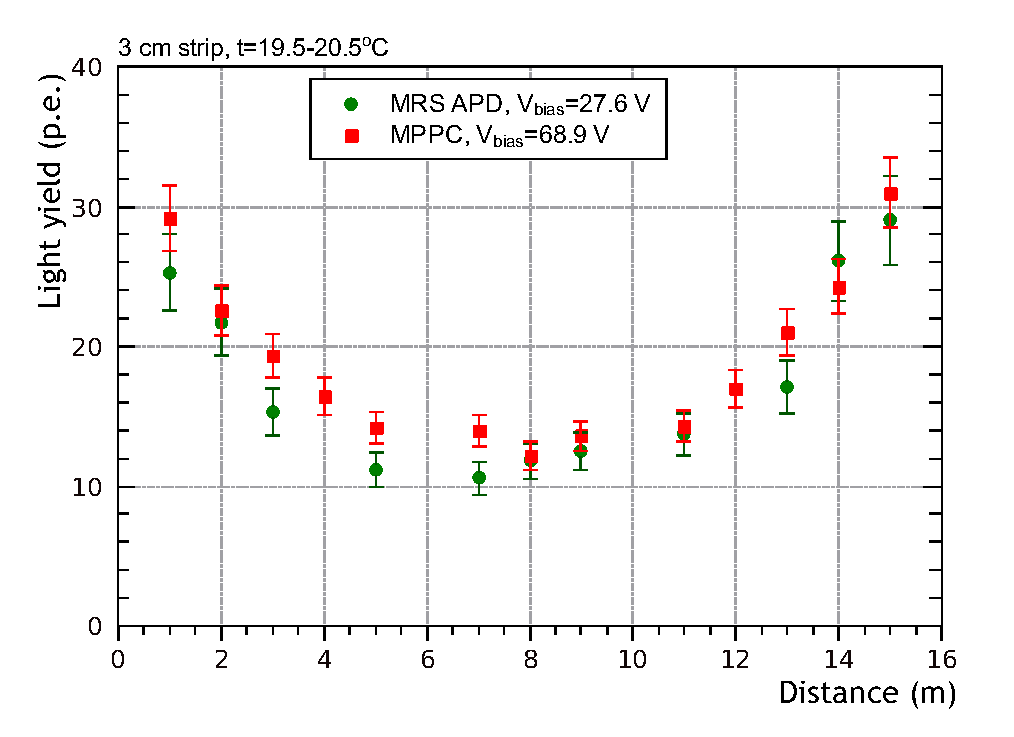
\includegraphics[width=11cm,angle=0]{figures/bar2.eps}
%\caption{Total light yield from both fiber ends  vs position along the Y11 fiber for the 3~cm wide bar.}
%\label{fig:bar2} 
%\end{figure}
%
%For example, one-end readout provides the light yield  of about 12-15 p.e. for a MIP passing the detector at the distance of 6 meters from the photosensor.  
The light yield of about 14 p.e. per a minimum ionizing particle ($\sim 7$ p.e./MeV for 1 cm thick bar) provides the efficiency  for detection of minimum ionizing particles of more than  99\% in an individual scintillator bar  for a detection threshold of 1.5 p.e.  Time resolution depends on the  light yield as $\sim 1/\sqrt{N_{p.e.}}$ where $N_{p.e.}-$ is the number of photoelectrons. For the l.y. of 20 p.e. the typical resolution  is obtained to be $\sigma ~ 1$ ns. Detectors with shorter WLS fibers were also tested. 
Light yield of the detector with a 5 m long WLS  Y11 fiber is shown in Fig.~\ref{fig:graph1}

\begin{figure}[htpb]
\centering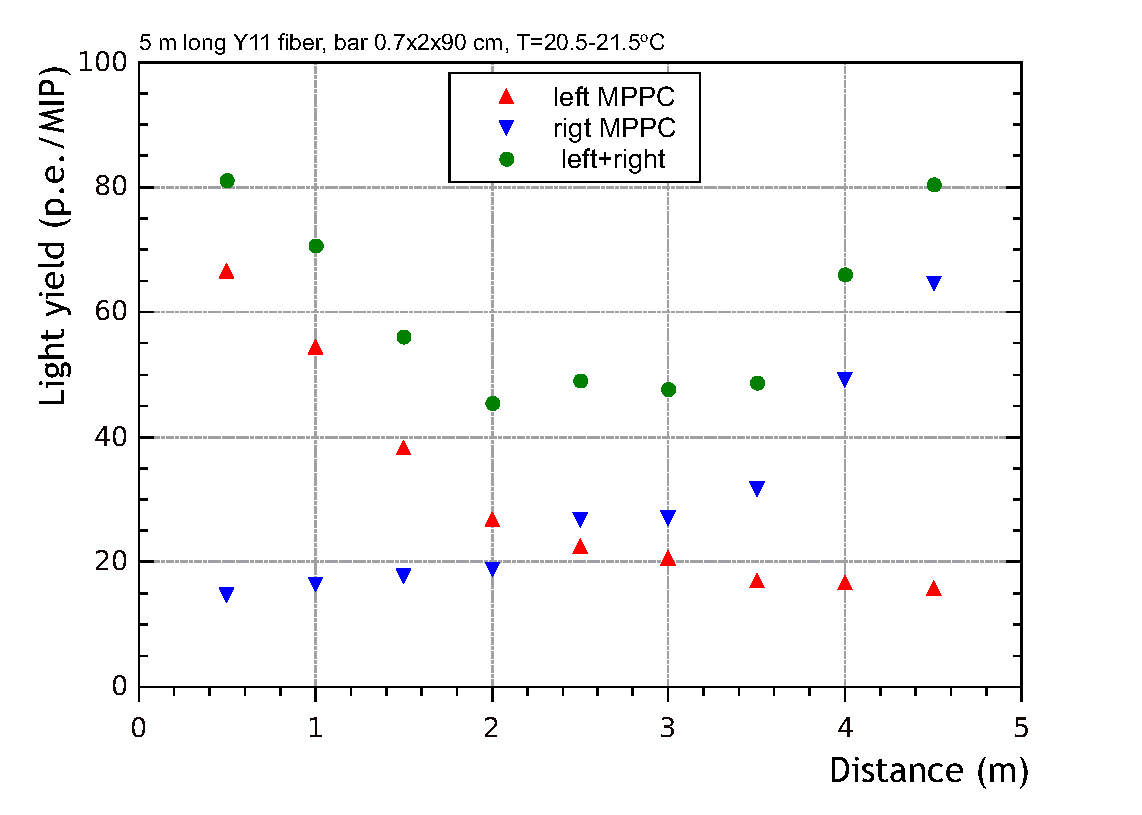
\includegraphics[width=9cm]{figures/Graph1.eps}
\caption{Light yield of a scintillator counter with  5 m long WLS  fiber vs position along the fiber. The T2K 667 pixel MPPC's were used in this measurement.}
\label{fig:graph1} 
\end{figure}
In this case, the minimum light yield of more that 40 p.e./MIP (sum of both ends) is obtained.

\subsubsection{Veto counters for \nuprism}

i%\begin{figure}[h!]
%\centering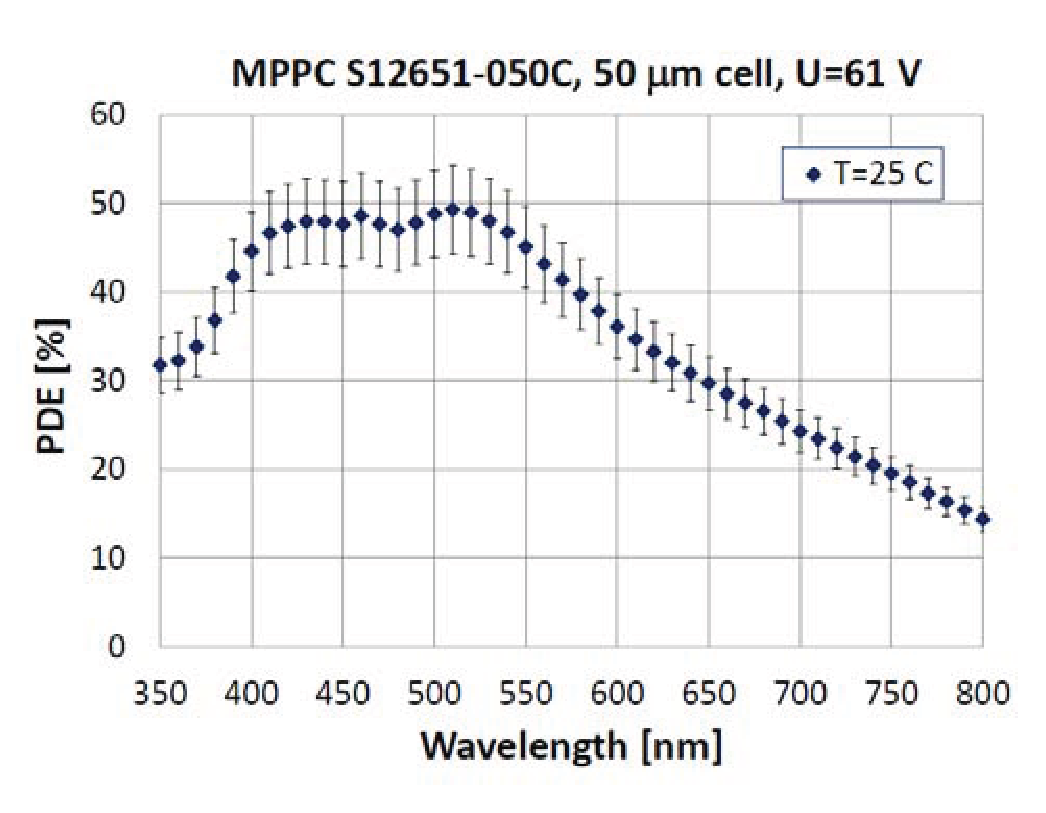
\includegraphics[width=10cm,angle=0]{figures/pde_new_mppc.eps}
%\caption{Photon detection efficiency  of the MPPC S12651-050C as a function of wavelength of the detected light~\cite{musienko_instr14}.}
%\label{fig:pde_new_mppc}
%\end{figure}


The excellent performance of the SMRD counters with one serpentine WLS fiber per counter gives a possibility to make a veto system using similar approach. One option is to construct the \nuprism veto system from scintillator counters,  each of 0.2 m$^2$.
%The geometry of one counter is shown in Figure~\ref{fig:nuprism_counter}.
%\begin{figure}[h!]
%\centering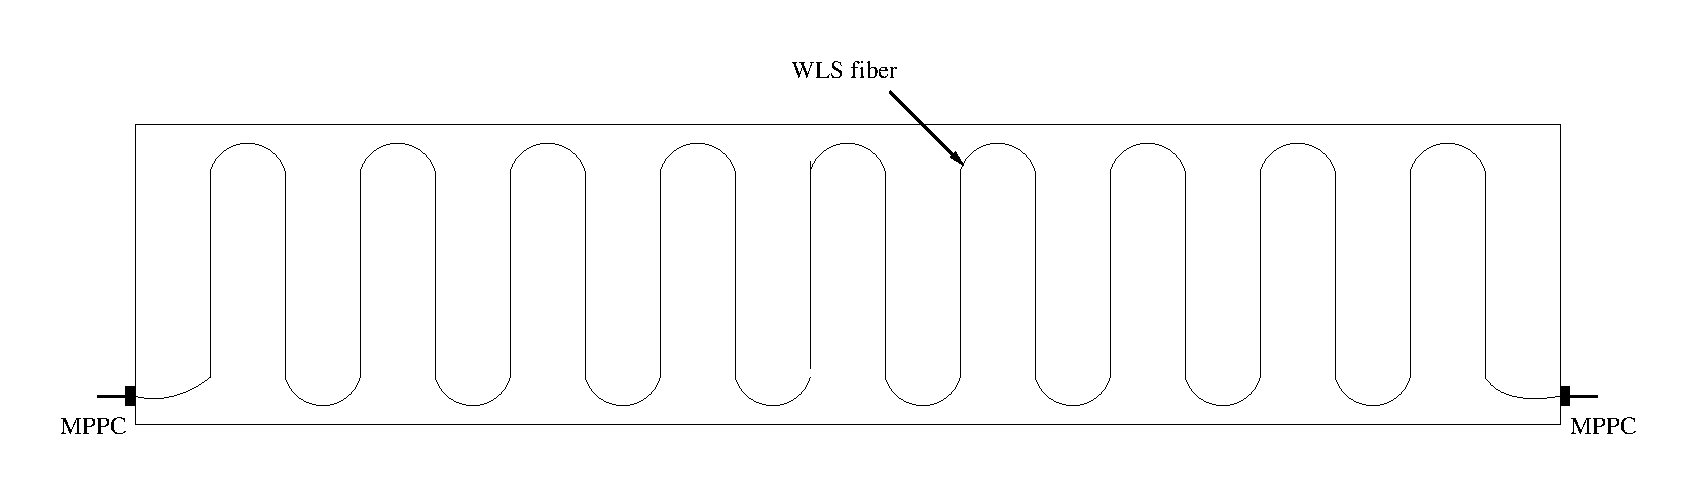
\includegraphics[width=13cm,angle=0]{figures/counter.eps}
%\caption{Drawing view of a scintillator counter for the \nuprism veto system.}
%\label{fig:nuprism_counter} 
%\end{figure}
One WLS Y11 S-type fiber is embedded in the extruded plastic slab of $2000 \times 200 \times 7 {\rm mm}^3$. Half-circles have the radius of 3 cm that allows to keep the performace of the fiber without loosing the transmission of the reemitted light along the fiber. A 6 m long Y11 fiber is readout on both ends by MPPC's. Taking into account the improved parameters of new MPPC's, for exmple, higher PDE, 
%as shown in Figure~\ref{fig:pde_new_mppc}, 
we can expect to obtain miminum light yield of 20-30 p.e./MIP and time resolution of about 1 ns for these detectors. More accurate information can be obtained after tests of the conter prototypes. 

\subsection{Photomultiplier Tubes}

%Section goals:
%\begin{itemize}
%\item 20 inch Hyper-K HPDs for OD
%\item 5 or 8 inch PMTs for ID (could be high QE or HPDs)
%\item discussion of cost
%\end{itemize}

The original T2K 2~km detector proposal used 8" PMTs to better match the granularity of the 20" PMTs used in the much-larger Super-K detector. The baseline design for the \nuprism detector is only 6~m in diameter and 10~m tall, which corresponds to 3,120 PMTs for 40\% photocathode coverage. This is significantly smaller than the 11,129 PMTs used at Super-K, so to improve the granularity of the detector, 5" PMTs are also being investigated, of which 7,385 PMTs would be required for 40\% coverage. Additional options such as avalanche photodiodes and high quantum efficiency coating are also being explored. Initial cost estimates from Hamamatsu for a wide variety of PMT configurations are given in the appendix.

\subsection{Electronics}

%\subsubsection{Electronics Overview}

Part of the goal of the \nuprism is to serve as a prototype for the Hyper-K.
We therefore want \nuprism to use a set of electronics that is as close as possible to the
electronics being proposed for Hyper-K.  Some of the key features of the Hyper-K electronics 
are the following:

\begin{itemize}
\item Front-end electronics will be placed in the water, as close as possible to the PMTs.
\item Front-end electronics are expected to find all hits above 0.25 PE and send all information 
about hits up to back-end electronics.  In back-end computers trigger decisions will be made using software.
No global triggers will be propagated to the front-end electronics.  
\item PMT digitization should provide 0.05 PE charge resolution, 0.25 ns timing resolution (for 1PE hits) and
0.1-1250 PE dynamic range.
\end{itemize}

We shall note various aspects of the \nuprism electronics where we may differ from
the default HK electronics plan.
In particular, one clearly different aspect of \nuprism will be the much higher rate of 
`pile-up' events during beam spills.  The rate of sand muon events entering the ID
may be as high as 0.19 per bunch.  
At minimum we therefore need electronics that can cleanly distinguish 
between PMT hits in different bunches; ie, hits with separation of order $\approx$ 600ns.  We may also 
want to have some capacity to distinguish between hits within a single bunch; ie hits that differ by 10s of ns.
This would be a more challenging requirement.


\subsubsection{FADC Digitization}\label{fadc_digitization}

Given this requirement for inter-bunch and intra-bunch hit resolution we propose using 
FADC digitization with basic digital signal processing in the front-end electronics.  
The basic scheme is as follows:  

\begin{enumerate}
\item The stretched/shaped PMT signal is fed into the FADC.
Use a standard commercial FADC, with sampling frequency between 80-500 MHz and 
12-16 bit resolution.
\item The digital output of FADC is fed into an FPGA (on the front-end electronic card), 
where we do basic digital pulse processing
(on the fly, at same rate as original digitization).  Digital pulse processing would involve the 
following:
\begin{itemize}
\item Finding PMT hits (for instance, by using simple threshold comparison).
\item Calculating the pulse time and charge.  
\end{itemize}
\item The digital pulse information is then transferred to the back-end electronics.  
We send different types of data depending on the pulse charge.

\end{enumerate}

It is worth emphasizing that the 
expected timing resolution using FADCs is not intrinsically limited by the sampling.  For instance, if you appropriately 
stretch and shape a PMT pulse you can easily achieve 0.25 ns timing resolution using a 100 MHz digitizer (ie a sample each 10 ns), as long
as you have high signal to noise ratio and a reasonable number of ADC samples on the leading and falling edges. 
We will explore the trade-offs involved in optimizing the performance of such a system in Section \ref{fadc_performance}.

\begin{figure*}[hptb]
\centering
%\resizebox{0.85\textwidth}{!} {
  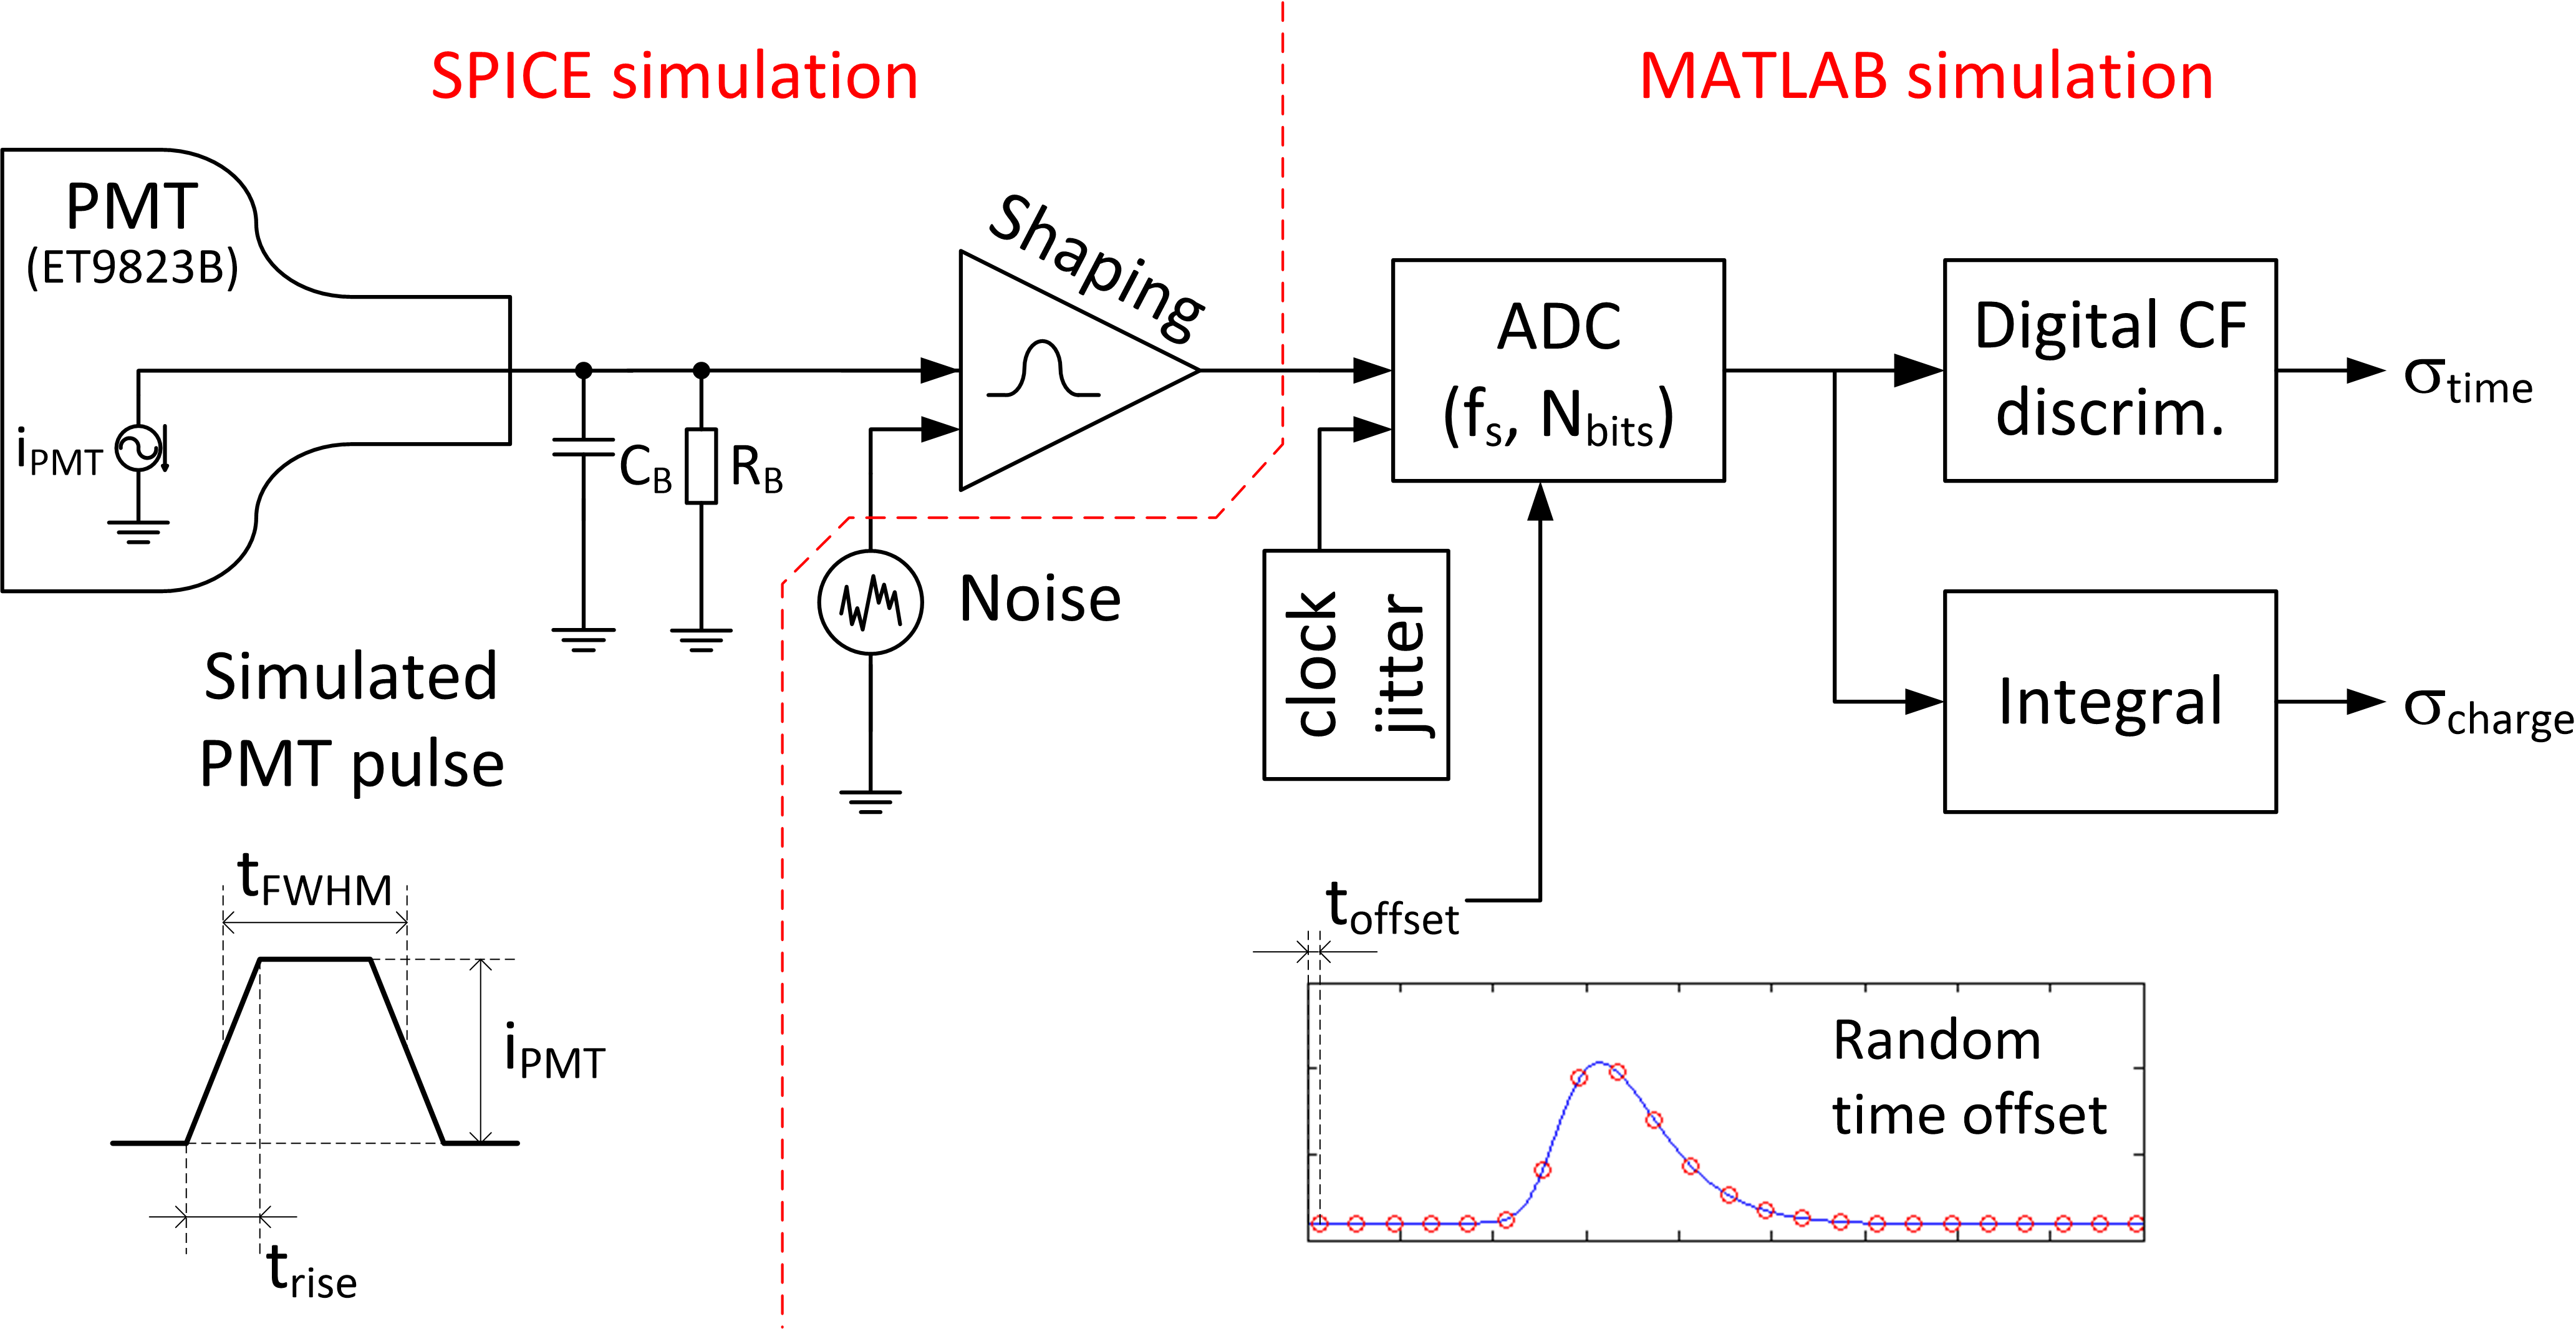
\includegraphics[width=0.7\linewidth]{figures/fadc_sim_setup.png}
%}
  \caption{Simulation setup for the study of the FADC performance.}
\label{fig:fadcSimSetup}
\end{figure*}

\subsubsection{Signal Conditioning And PMT HV}\label{fadc_signal_conditioning}

We propose to use differential transmission in order to deliver signals from the PMT bases to the digitization board. An advantage of such a solution is that, in principle, it would allow us to use a standard unshielded twisted pair cable, while still maintaining fairly good immunity to pickup of electromagnetic interference. The base of the PMT would contain shaping circuitry, which would stretch PMT signals, limiting their bandwidth to match FADC requirements and converting them into a symmetric form, suitable for transmission via a twisted pair cable. Preliminary studies show that signal shaping using a 5-th order Bessel-type low pass filter should provide satisfactory results. 

One of the design goals for the \nuprism is minimization of the amount of necessary cables. As such, it would be advisable to use a single cable to provide both high voltage to the PMT and to transmit the signal from the PMT base to the digitization board. Therefore, the preferable solution would be to synthesize the high voltage directly on the PMT base, from a 48-200 V DC supply, using either a commercial high voltage module or a custom designed voltage multiplier structure. This way, power to the PMT base could be delivered via an additional twisted pair of the same cable that would be used to transmit the shaped PMT signal. The slow control link necessary to tune the high voltage for specific PMT could be realized via a DC power line, thus avoiding the need to use additional cables. In any case, it should be emphasized that the details of the PMT HV implementation will depend strongly on the exact PMTs that are chosen.


\subsubsection{Digitization Performance/Optimization}\label{fadc_performance}

There is a strong inter-dependance of the digitization performance on the signal conditioning, type and
parameter of the chosen analog-to-digital converter (ADC) and the applied signal processing algorithms. The key parameters here are the speed and accuracy of the ADC\ as well as signal to noise ratio (SNR) of the whole system. Cost-wise, it would be best to use as slow and as least accurate ADC as possible while still meeting the performance requirements. Therefore, a Monte-Carlo study has been performed in order to estimate impact of the electronics chain on the overall system performance.  

\begin{figure}[htpb]
\centering
%\resizebox{0.99\textwidth}{!} {
  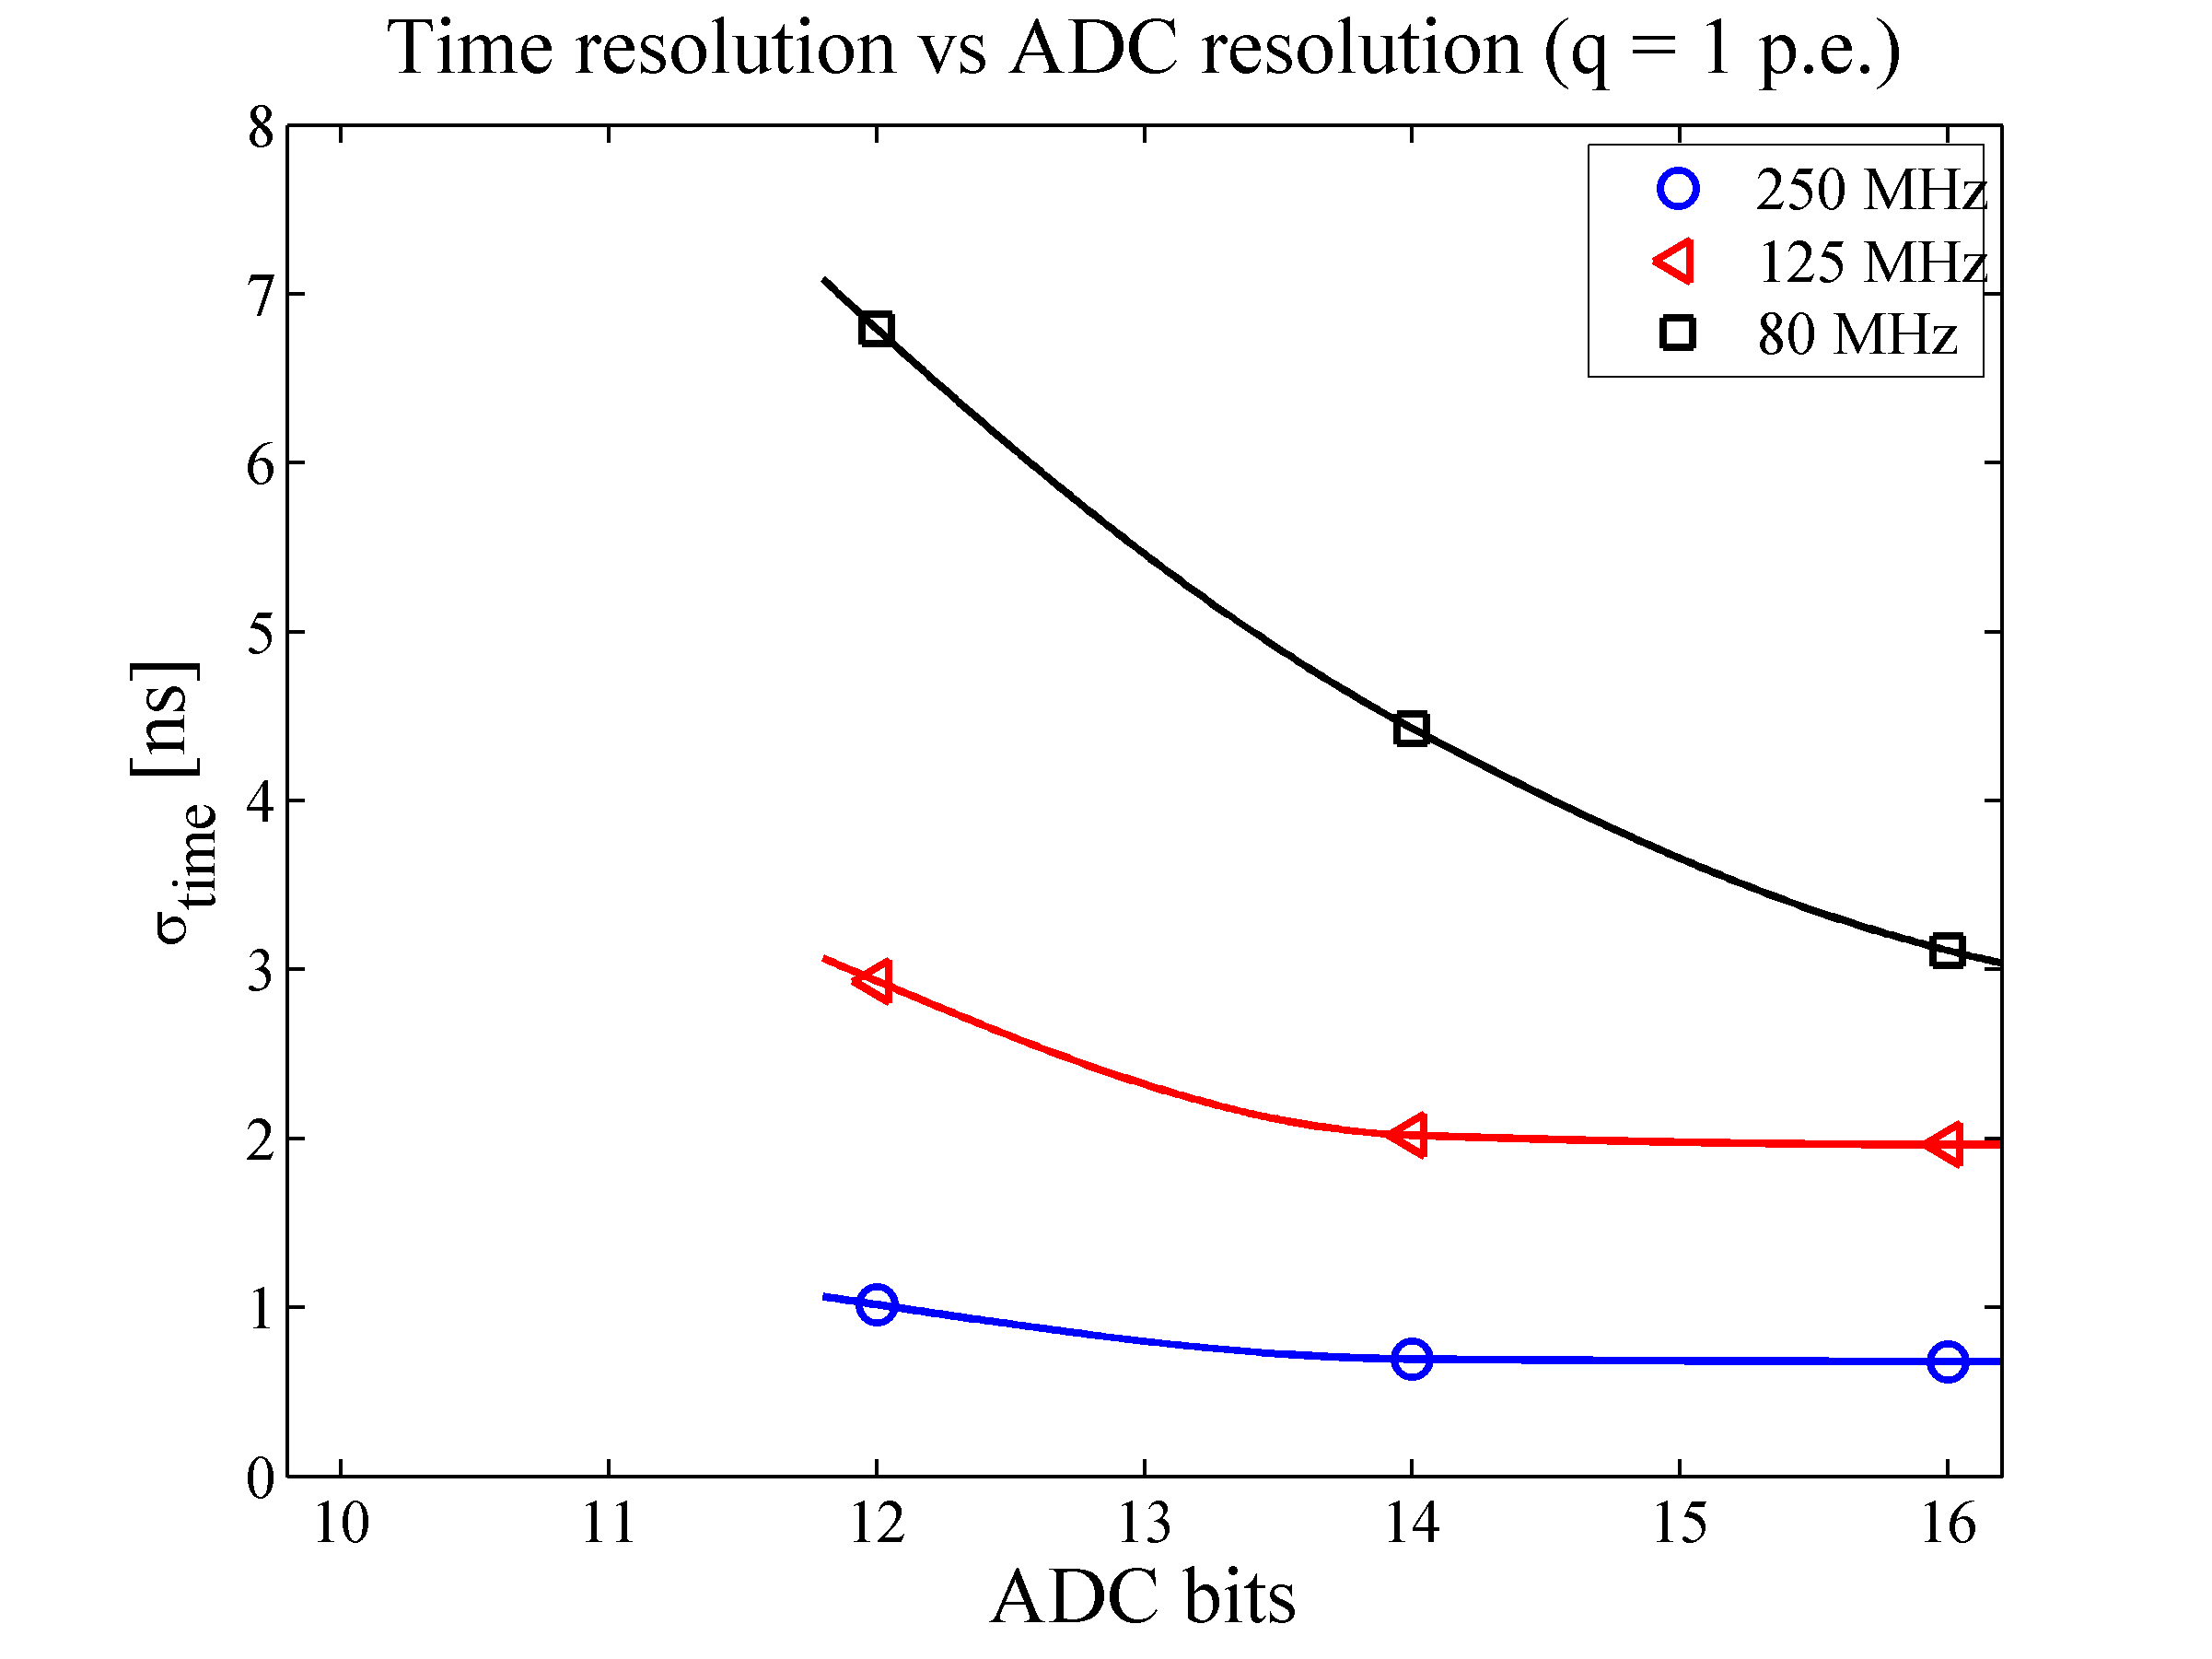
\includegraphics[width=9cm]{figures/time_vs_bits-dyn_2000pe-pls_1pe.png}
  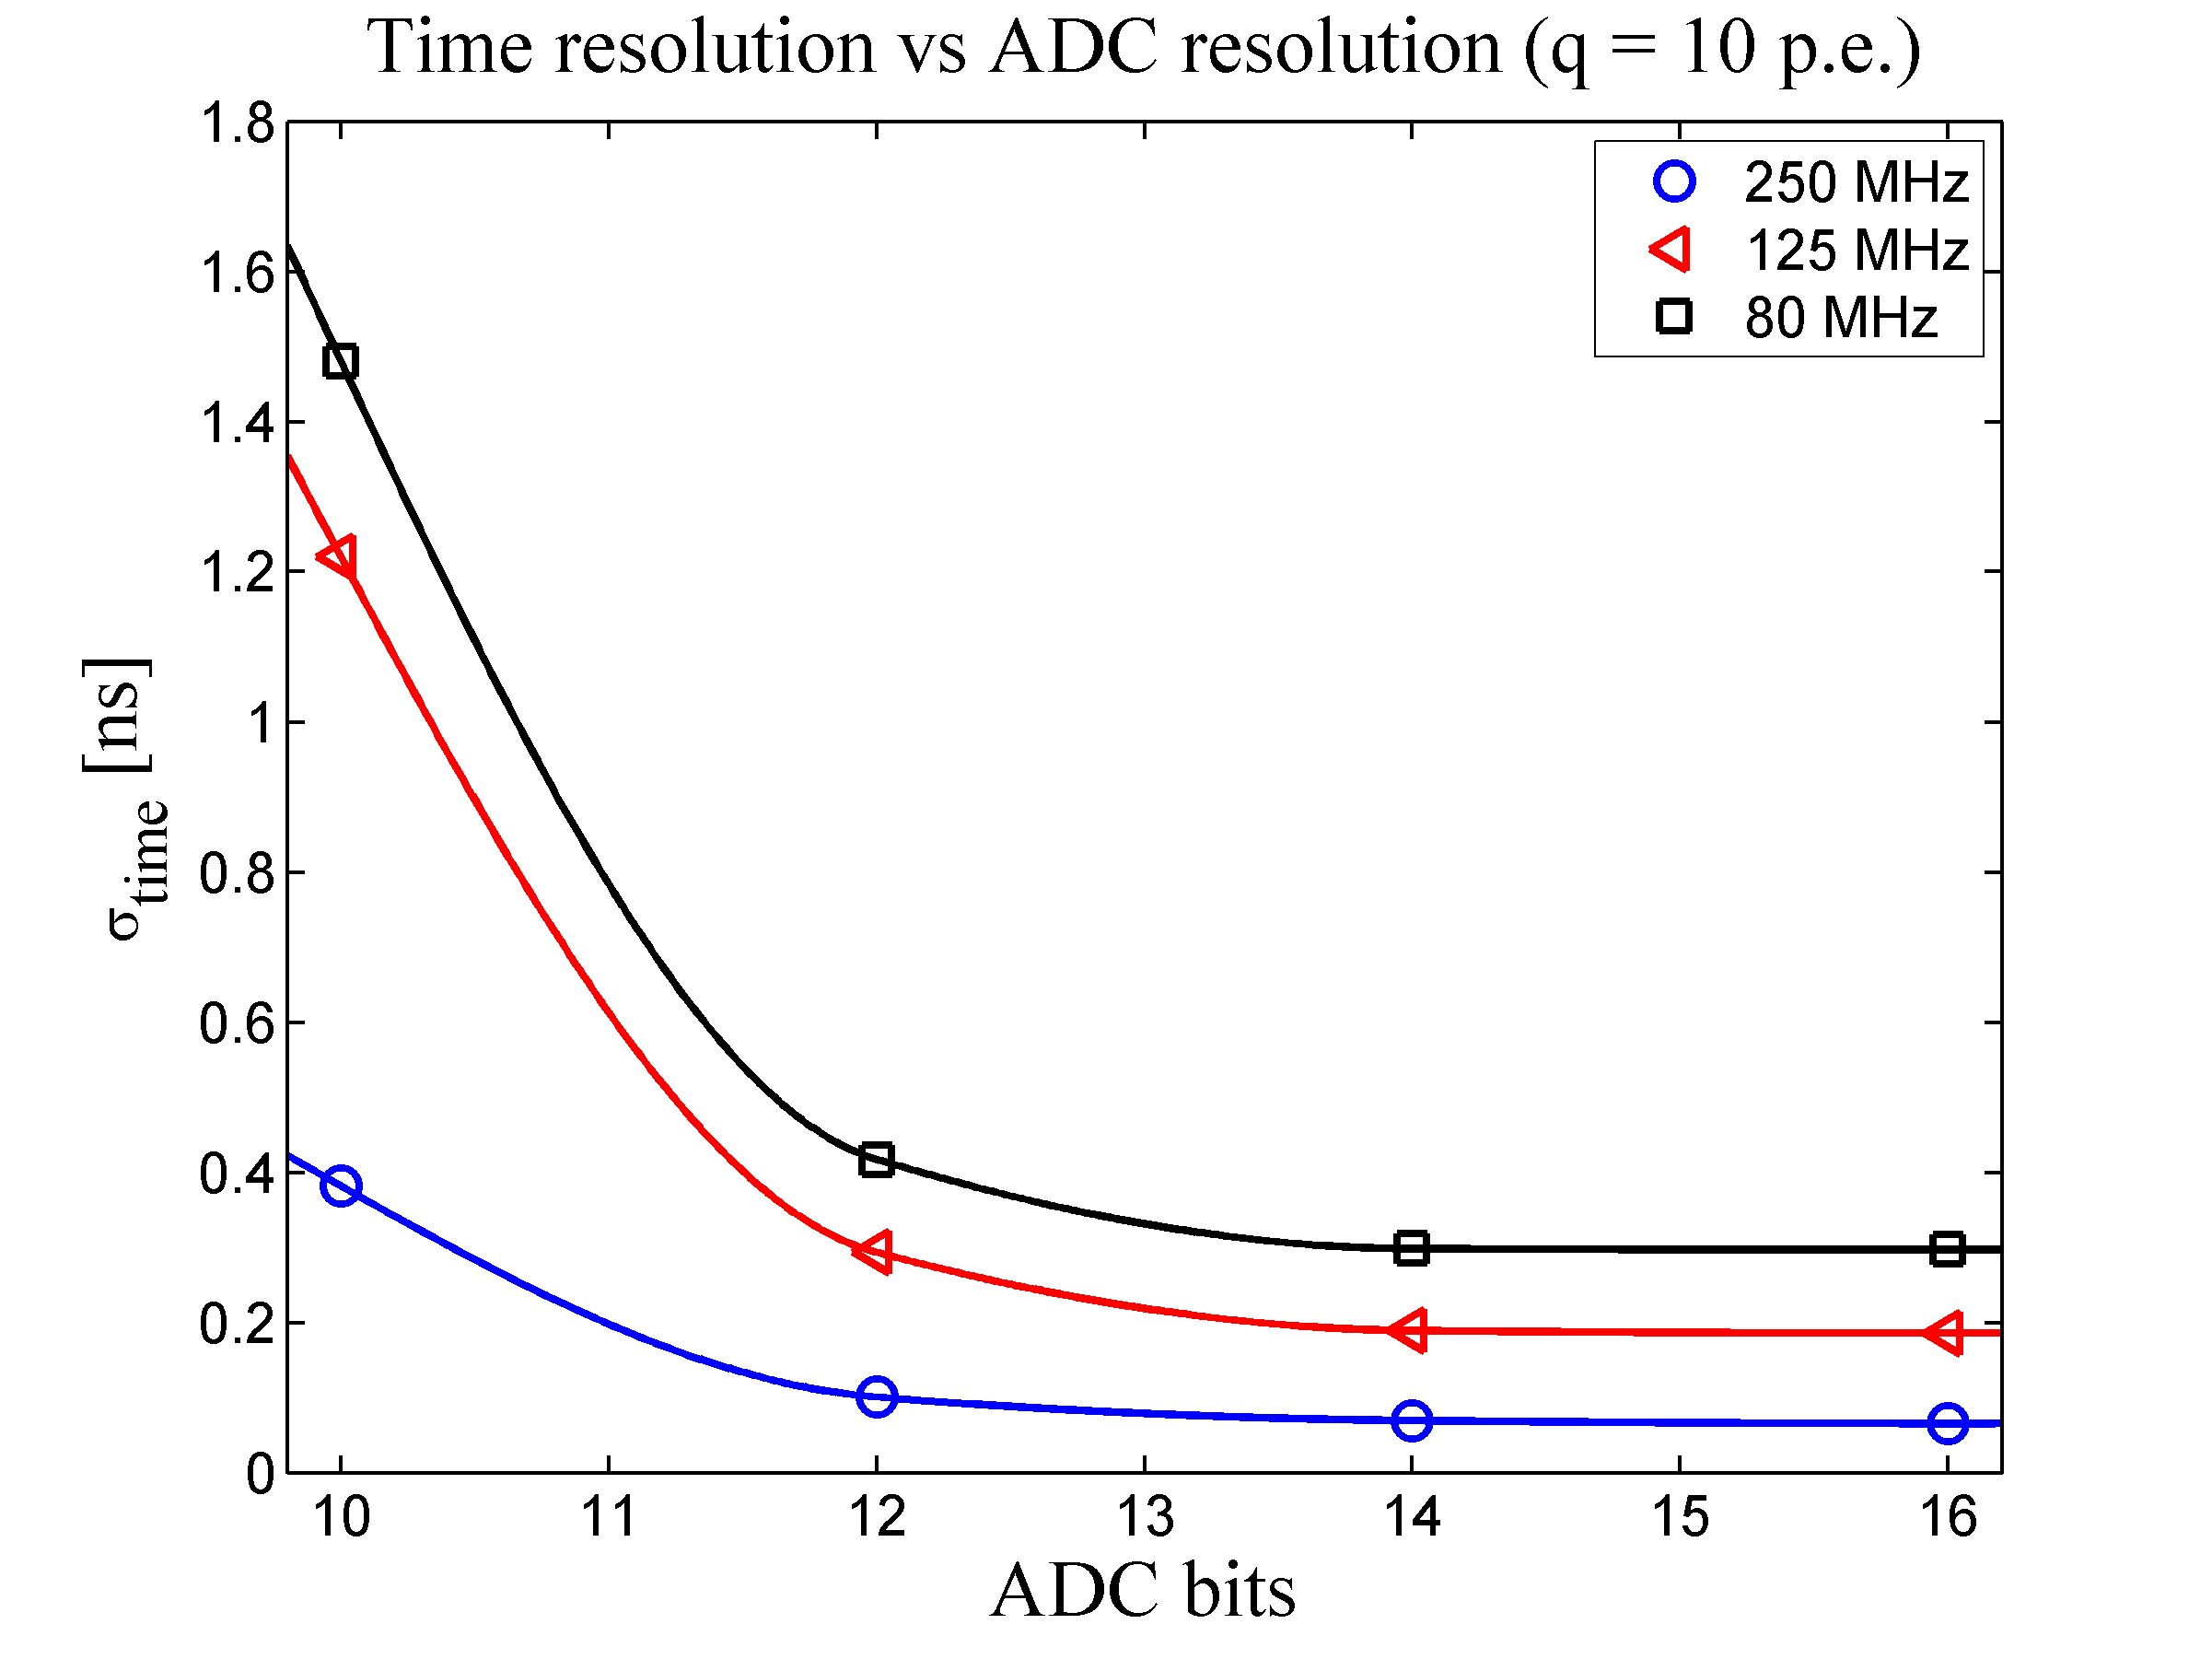
\includegraphics[width=9cm]{figures/time_vs_bits-dyn_2000pe-pls_10pe.png}
%}
  \caption{Estimated timing resolution for FADC digitization, as a function of sampling frequency and ADC precision.  The top plot is for 1PE pulses; bottom is for 10PE pulses.}
\label{fig:timing_vs_dyn}
\end{figure}

\begin{figure}[htpb]
\centering
%\resizebox{0.99\textwidth}{!} {
  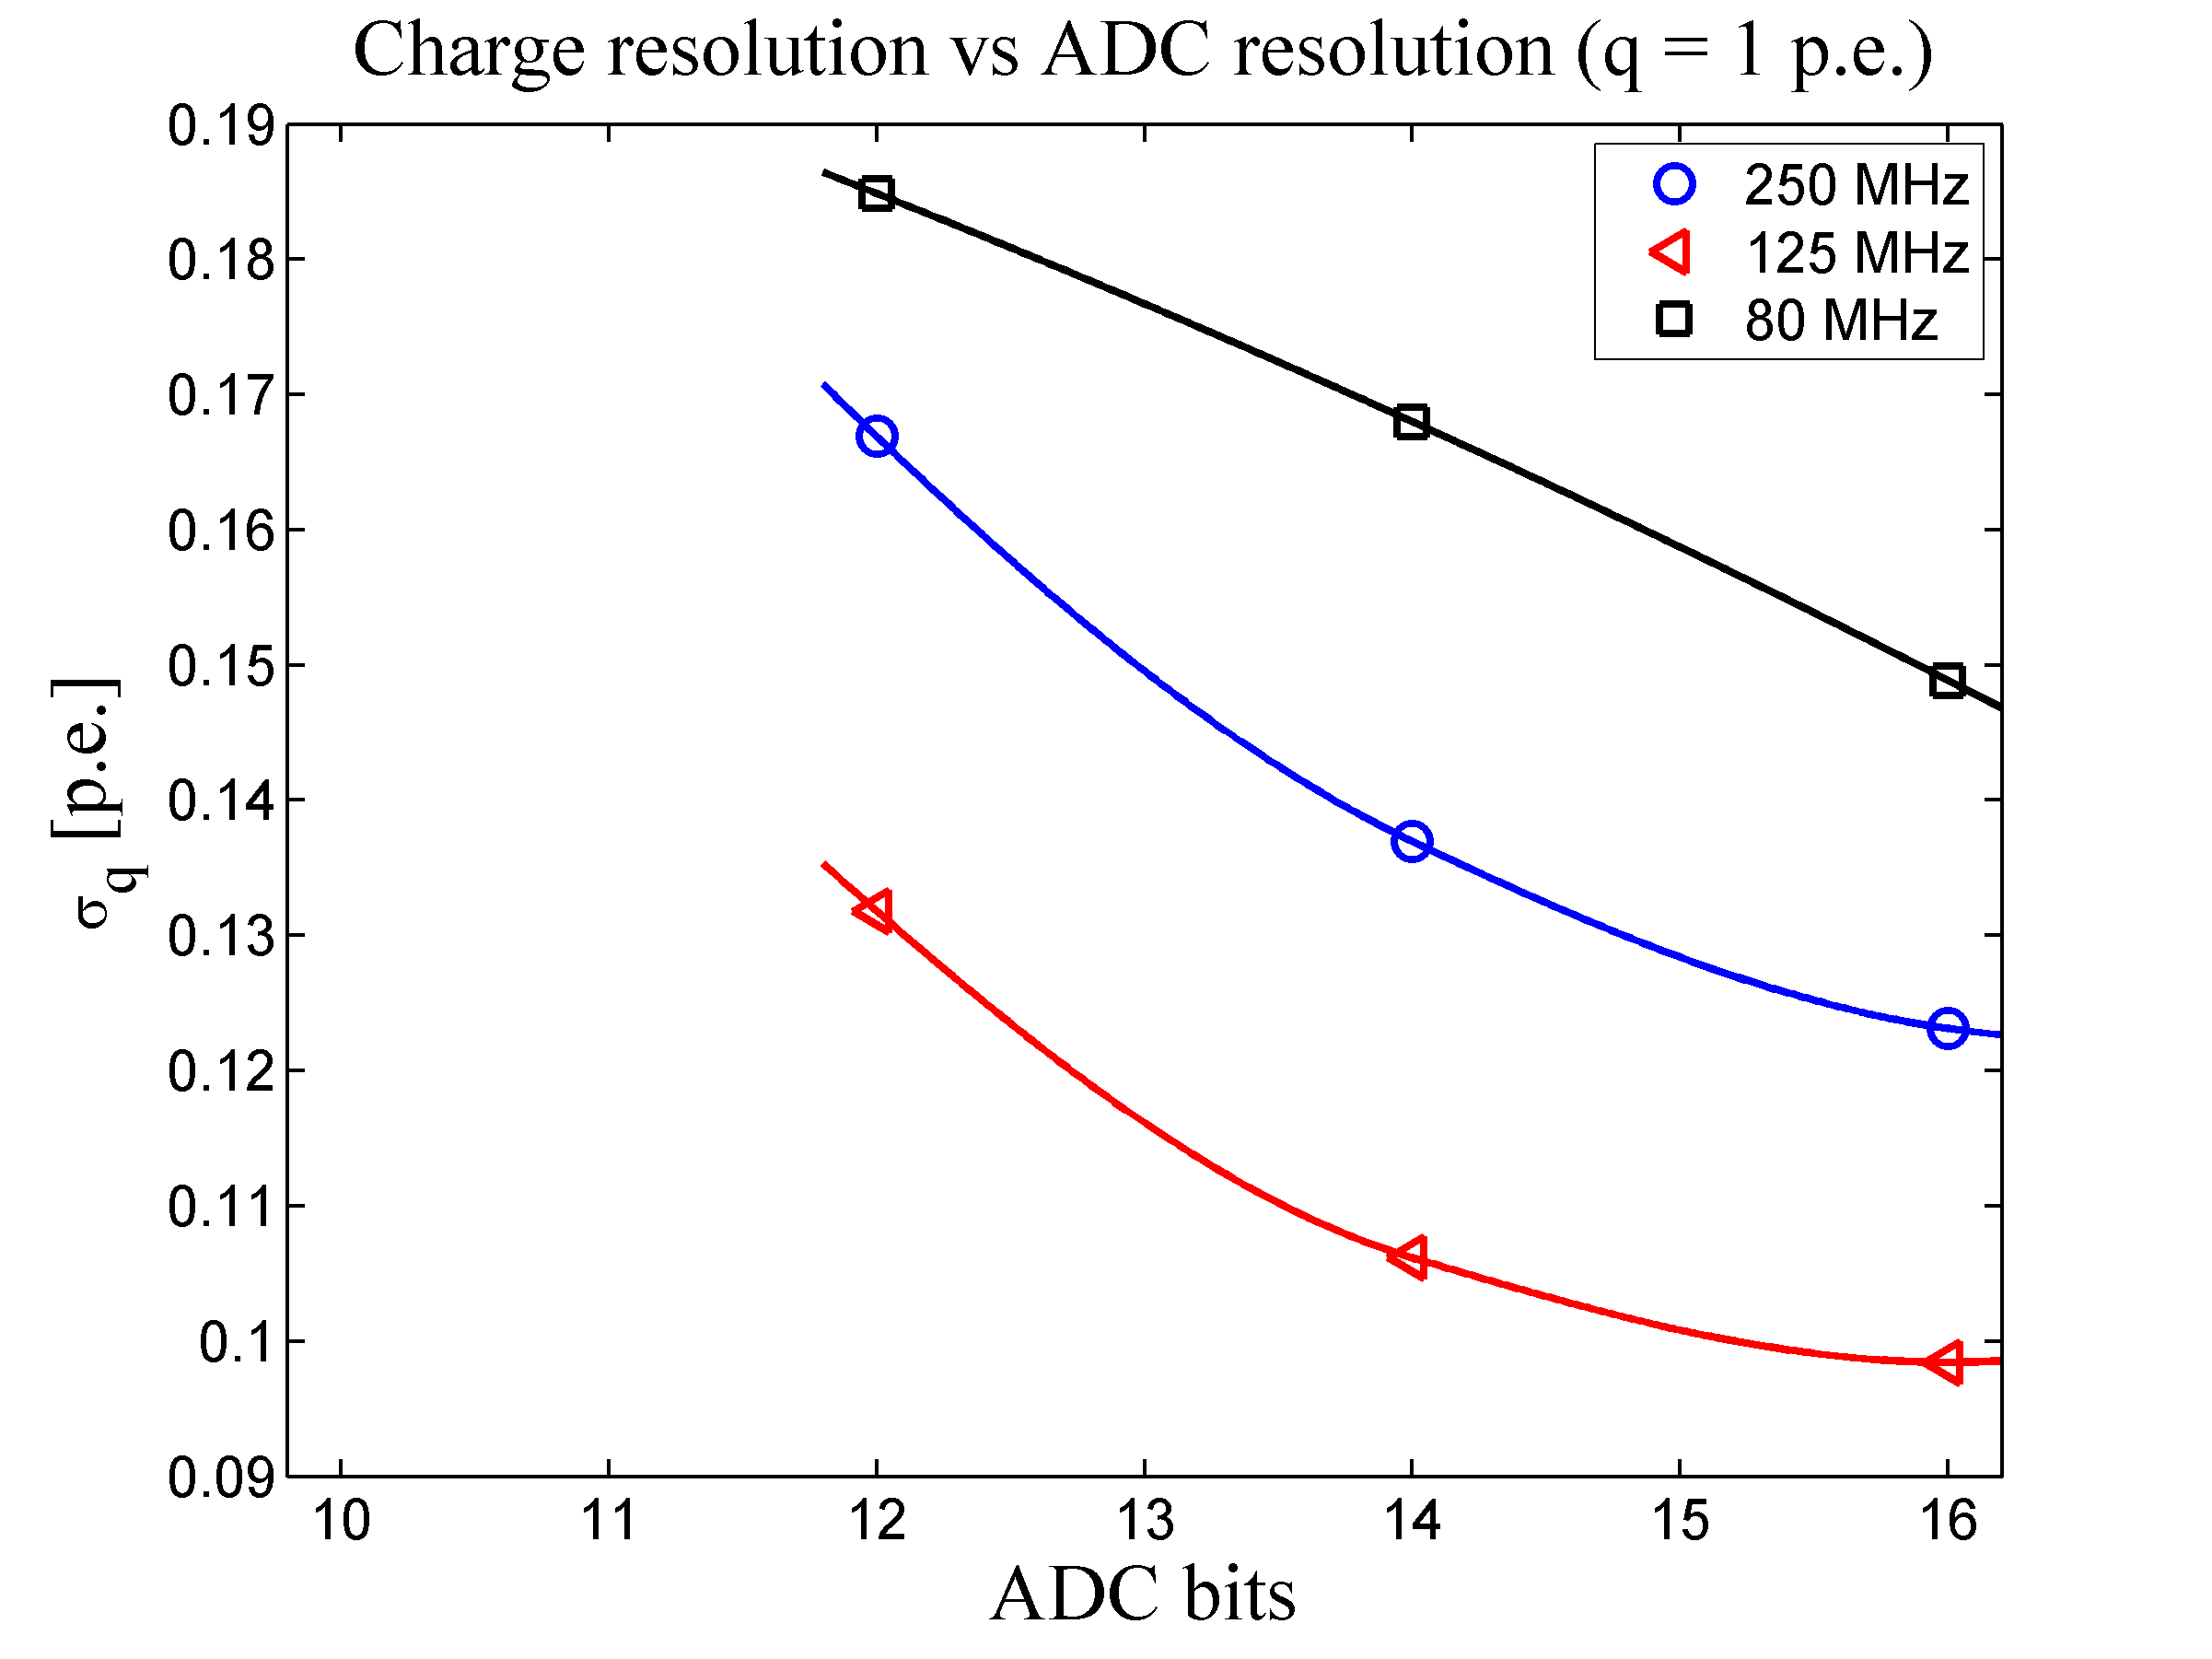
\includegraphics[width=9cm]{figures/charge_vs_bits-dyn_2000pe-pls_1pe.png}
  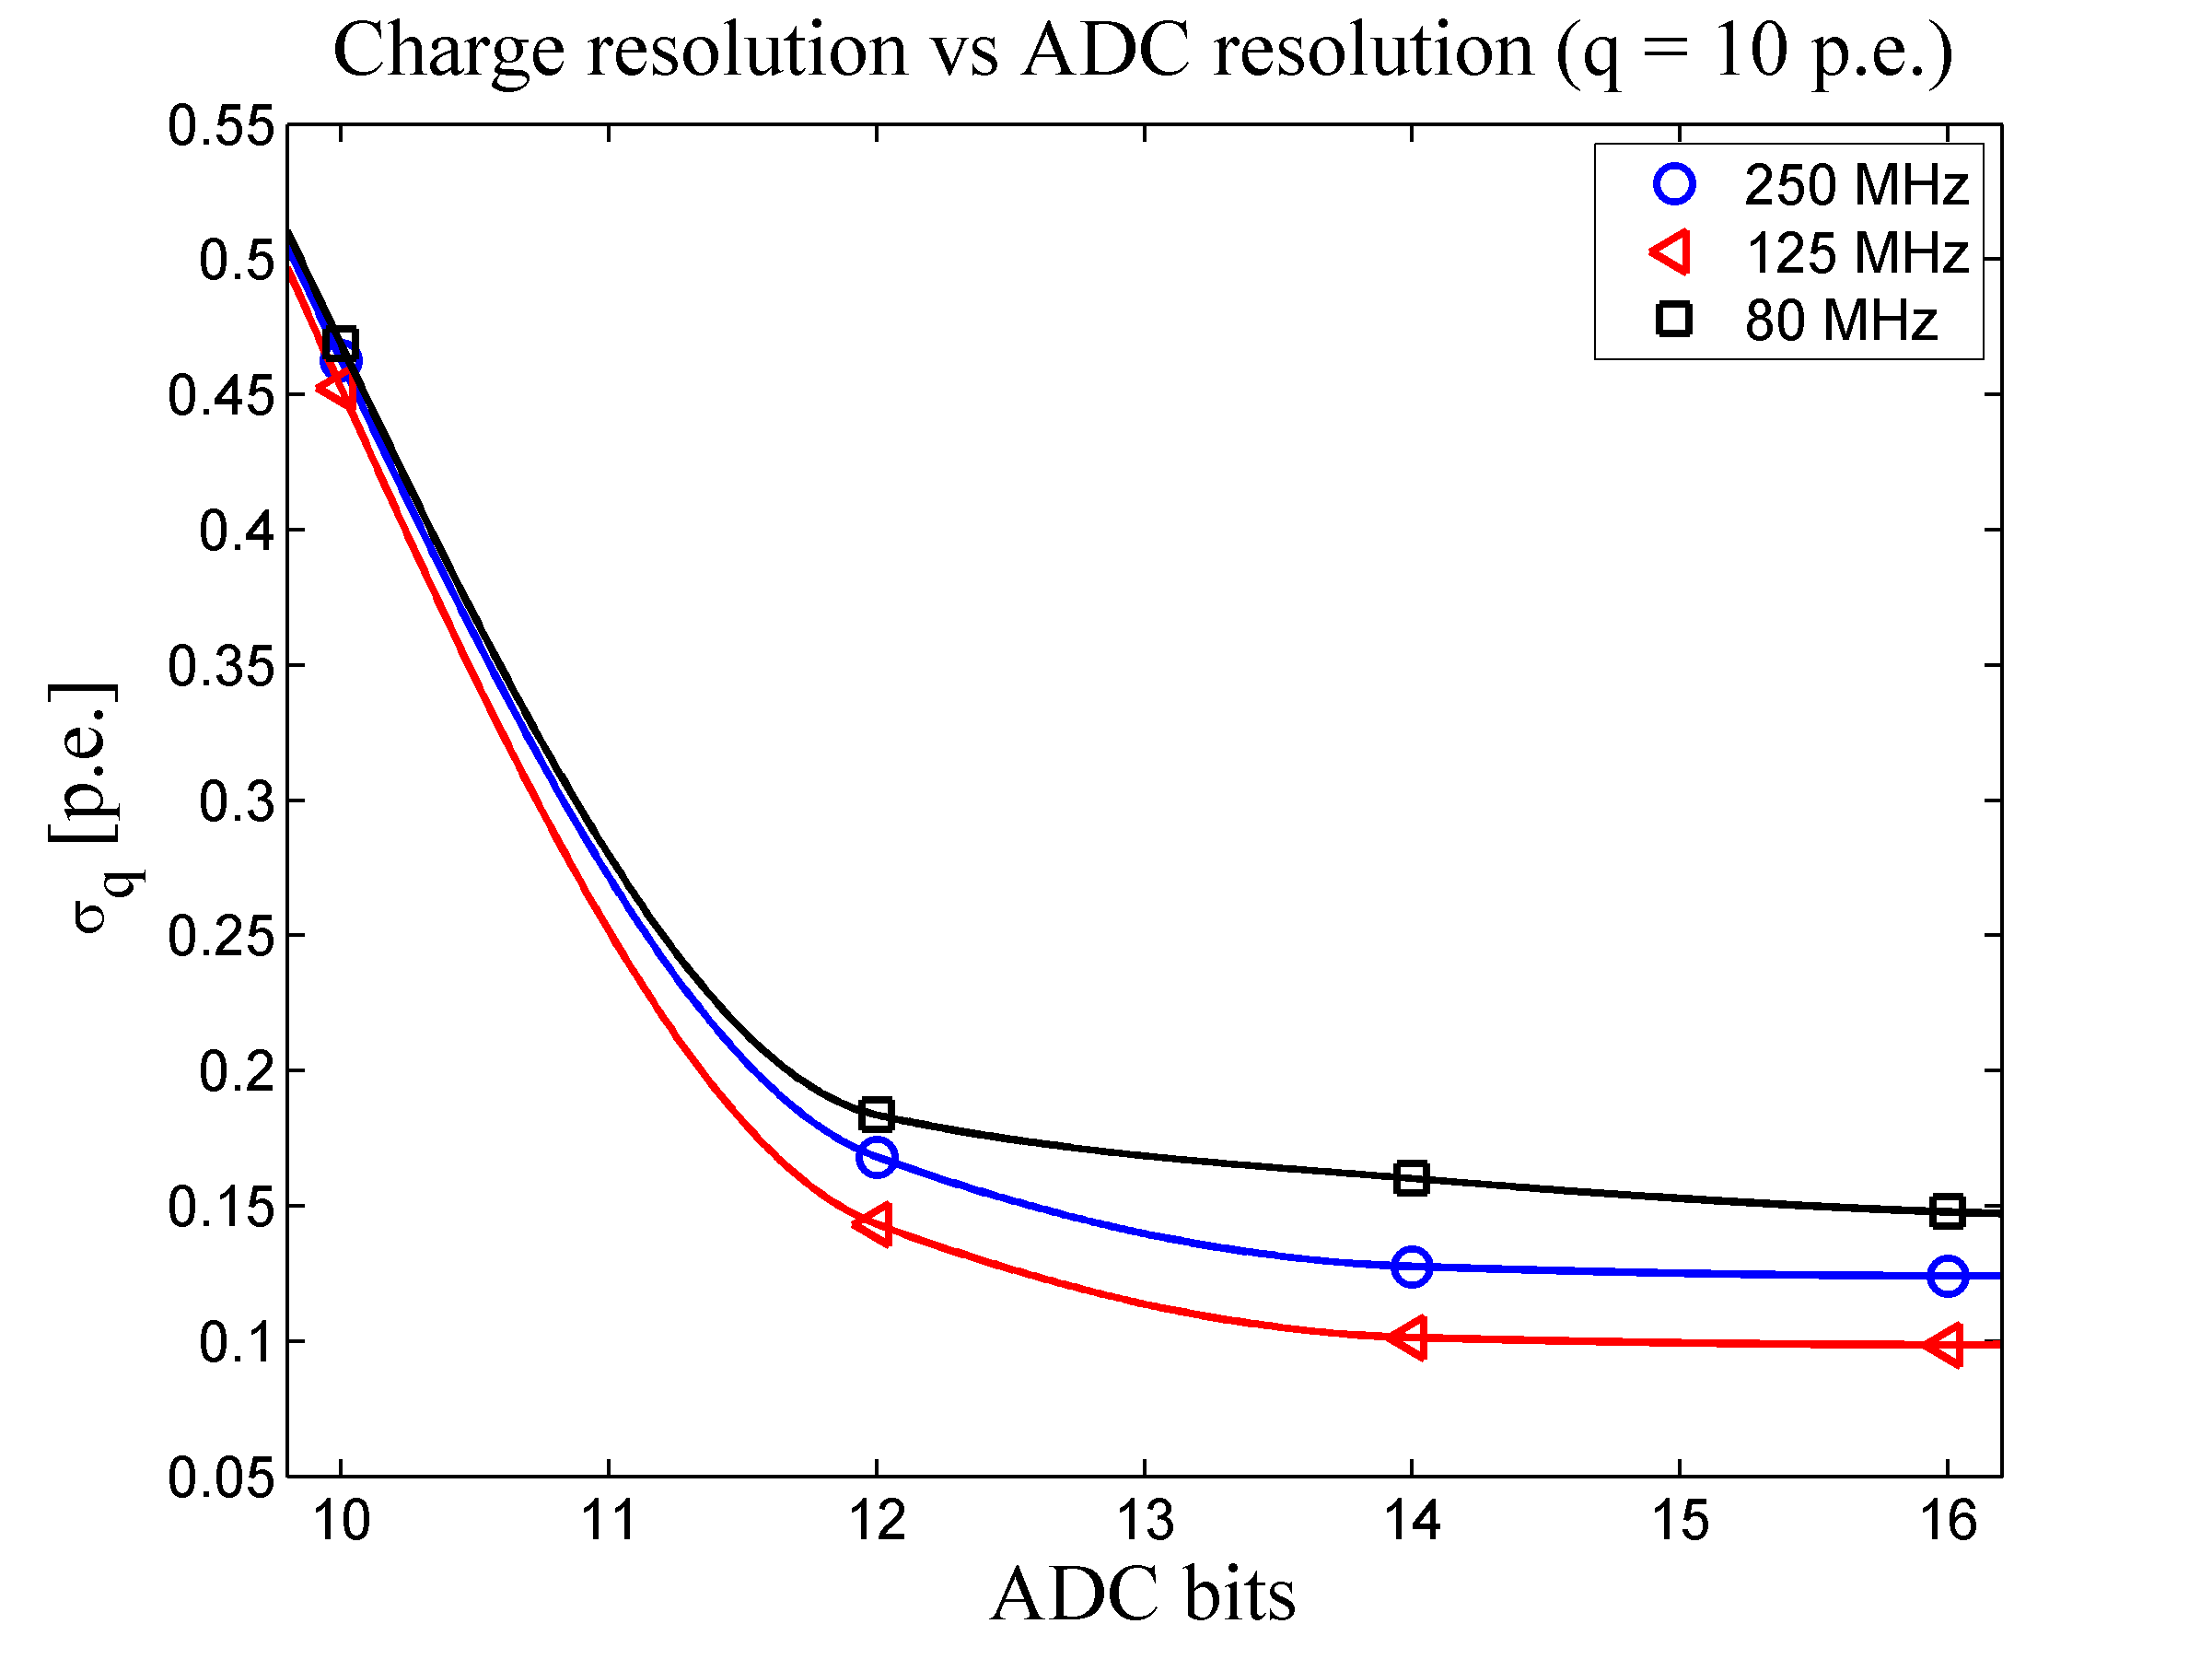
\includegraphics[width=9cm]{figures/charge_vs_bits-dyn_2000pe-pls_10pe.png}
%}
  \caption{Estimated Charge resolution for FADC digitization, as a function of sampling frequency and ADC precision.  The top plot is for 1PE pulses; bottom is for 10PE pulses.}
\label{fig:charge_vs_dyn}
\end{figure}


Simulation setup is presented in Fig.~\ref{fig:fadcSimSetup}. The photomultiplier has been simulated as a current source (\(i_{PMT}\)), connected in parallel with a base resistor \(R_{B}\)  and a capacitor \(C_{B}\), which together form the first pole of the shaping low-pass filter. Both the \(R_{B}\) and the \(C_{B}\) were chosen to fulfil the dynamic range requirement while maintaining the best possible signal to noise ratio,  i.e. to provide the highest possible PMT signal for maximum pulse charge (2000 p.e.) without saturating the amplifiers. The PMT current pulse waveform was approximated using a trapezoid pulse, with timing parameters (\(t_{rise}\), \(t_{FWHM}\)) corresponding to manufacturer specification given in the PMT datasheet. The rise and fall times were assumed to be equal. Given the time constants of the shaper, the PMT pulse can be treated as a delta function. 

The output of the shaper's response simulated in the SPICE   program was then sampled, quantized and subsequently analyzed using a digital Constant Fraction Discrimator (CFD), modeled in MATLAB.
Using the result of the CFD,
the difference between the calculated time and the real time was calculated, as well as the difference of calculated pulse charge and the real pulse charge.
A summary of the results is presented in Figures \ref{fig:charge_vs_dyn} and \ref{fig:timing_vs_dyn}.  As can be seen, there is some
difficulty in achieving the desired timing and charge resolution for the 1 p.e. pulses, which is due to poor signal to noise ratio. In particular, even with a 16-bit, 250MHz sampling we can only achieve approx. 0.8 ns timing resolution for the single p.e. (compared to the desired 0.25ns resolution).

As such, further studies are ongoing in order to find a working solution. The considered options include splitting the signal from the PMTs to separate high and low gain
branches which would then be digitized by their own ADCs. Other possibilities include dropping the linearity requirement for the PMT response to large number of photons and running it at higher gain. A significant effort is also foreseen to optimize signal processing algorithms for poor SNR conditions, in particular an adoption of matched filtering approach is planned.


\subsection{Water System}

Starting with the very first large-scale Water Cherenkov detector -- the
Irvine Michigan Brookhaven [IMB] proton decay experiment, which began
taking data in the early 1980's -- exceptional water clarity has been of
key importance for massive devices of this kind.  There is
little benefit in making a very large detector unless the target mass
contained within the detector can be efficiently observed.  Good water
quality has two main advantages: the light generated by physics
interactions in the water can propagate long distances with minimal
attenuation until it is collected by photomultiplier tubes or other
technologies, aiding accurate energy reconstruction, and the light can traverse
these distances (10's of meters) with minimal scattering, which aids
in the precise reconstruction of event vertices.

The strategy employed to create
kilotons of extremely clear water has been to remove all suspended solids,
dissolved gases, ions, and biologics from solution via a series of
filtration elements.  These include microfiltration filters, degasifiers
(vacuum and/or membrane type), reverse osmosis membranes [RO],
de-ionization resins [DI], and exposure to intense ultraviolet light [UV].

These water systems typically run in one of two modes: fill or
recirculation.  During the fill mode, water supplied by the local
municipality or ground water in the vicinity of the experiment is first brought
up to ultrapure levels and then injected into the detector.  The capacity of the water 
system, along with availability of water, defines how long it will take to fill the detector.  
During recirculation mode, already high-quality water from the detector is
continuously passed through the filtration system and returned to the
detector after being cleaned even further. This is necessary as transparency-impairing
materials are steadily leaching into the chemically active ultrapure water.  In addition, 
during the process of filtration the water is typically chilled to further
impede biological growth, with the added benefit of simultaneously reducing PMT 
dark noise which is typically strongly temperature dependent.

In the current baseline design, \nuprism will have interior dimensions ten times smaller than Super-K.
It is therefore possible that a commensurately less powerful water filtration system would be able to
provide sufficient water transparency.  Nevertheless, for now we will base our initial system design 
and flow rates on water systems known to have worked and produced useful physics in the past.

Following this approach, a baseline design and cost estimate for the \nuprism water system 
has been prepared.  The primary components described above are represented graphically in 
Figure~\ref{water:water}. This system will be capable of filling the detector at a rate of 
6.3 tons/hour, such that a complete fill can be completed in one month of operations.  
It will be capable of recirculating the water at a rate of  6.3 tons/hour through the entire system 
plus an additional 22.8 tons/hour through what is known as a secondary "fast recirculation" 
path which trades some filtration components for faster overall flow. The combination of 
complete cleaning and fast recirculation has been shown at previous experiments (including 
the K2K one kiloton near detector) to be the most cost-effective way of achieving the desired 
water transparencies.  A preliminary cost estimate for this baseline water system from South Coast Water in the is \$350,000, including shipping, duties, and installation at the detector site.

\begin{figure}[htpb]
     \begin{center}
       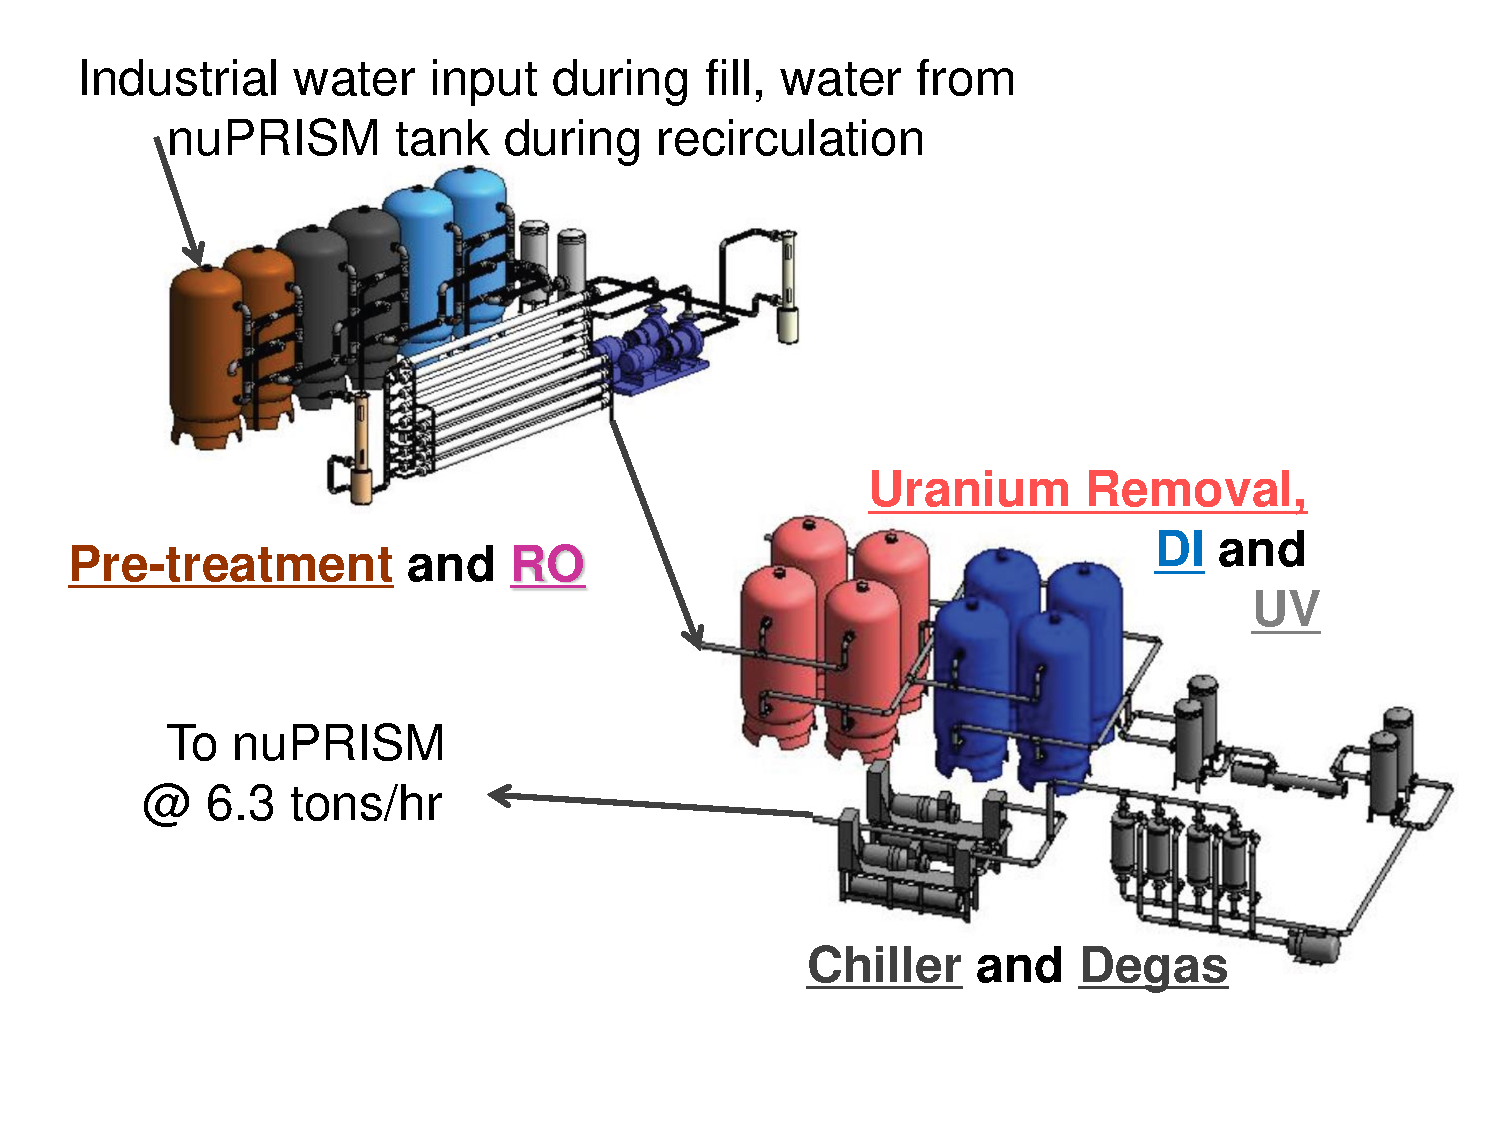
\includegraphics[width=9cm]{figures/nuPRISM_water.pdf}
       \caption{A preliminary baseline design of the \nuprism water system.}
       \label{water:water}
     \end{center}
\end{figure}


\subsubsection{Gd option}

If it is decided to add 0.2\% gadolinium sulfate by mass to 
Super-Kamiokande in order to provide efficient tagging 
of neutrons in water, it will likely be useful for a near detector at Tokai to also be 
Gd-loaded such that the responses of both detectors are as similar as possible.  As a large 
water Cherenkov detector, \nuprism is a natural candidate for eventual Gd-loading.  Therefore, 
the implications this has on the water system design must be taken into account.

Over the past decade there have been focused R\&D programs both in the US and Japan aimed 
at devising a method capable of maintaining the exceptional water transparency discussed 
above, while at the same time maintaining the desired level of dissolved gadolinium in solution.  
In other words, somehow the water must be continuously recirculated and cleaned of 
everything {\em except} gadolinium sulfate.

Starting in 2007 with a 0.2~ton/hour prototype at the University of California, Irvine, since 2009 
the Kamioka-based EGADS (Evaluating Gadolinium's Action on Detector Systems) project 
has shown that such a selective water filtration technology -- known as a ''molecular band-pass
filter''  and schematically shown in  Figure~\ref{water:bandpass} -- is feasible at  3~tons/hour.  
As the EGADS design is modular and uses off-the-shelf and readily available equipment, albeit 
in novel ways, scaling it up from the current 3~tons/hour to 60~tons/hour for Super-Kamiokande, 
is straightforward, while scaling to \nuprism's 6.3 tons/hours would be trivial.

\begin{figure}[htpb]
     \begin{center}
       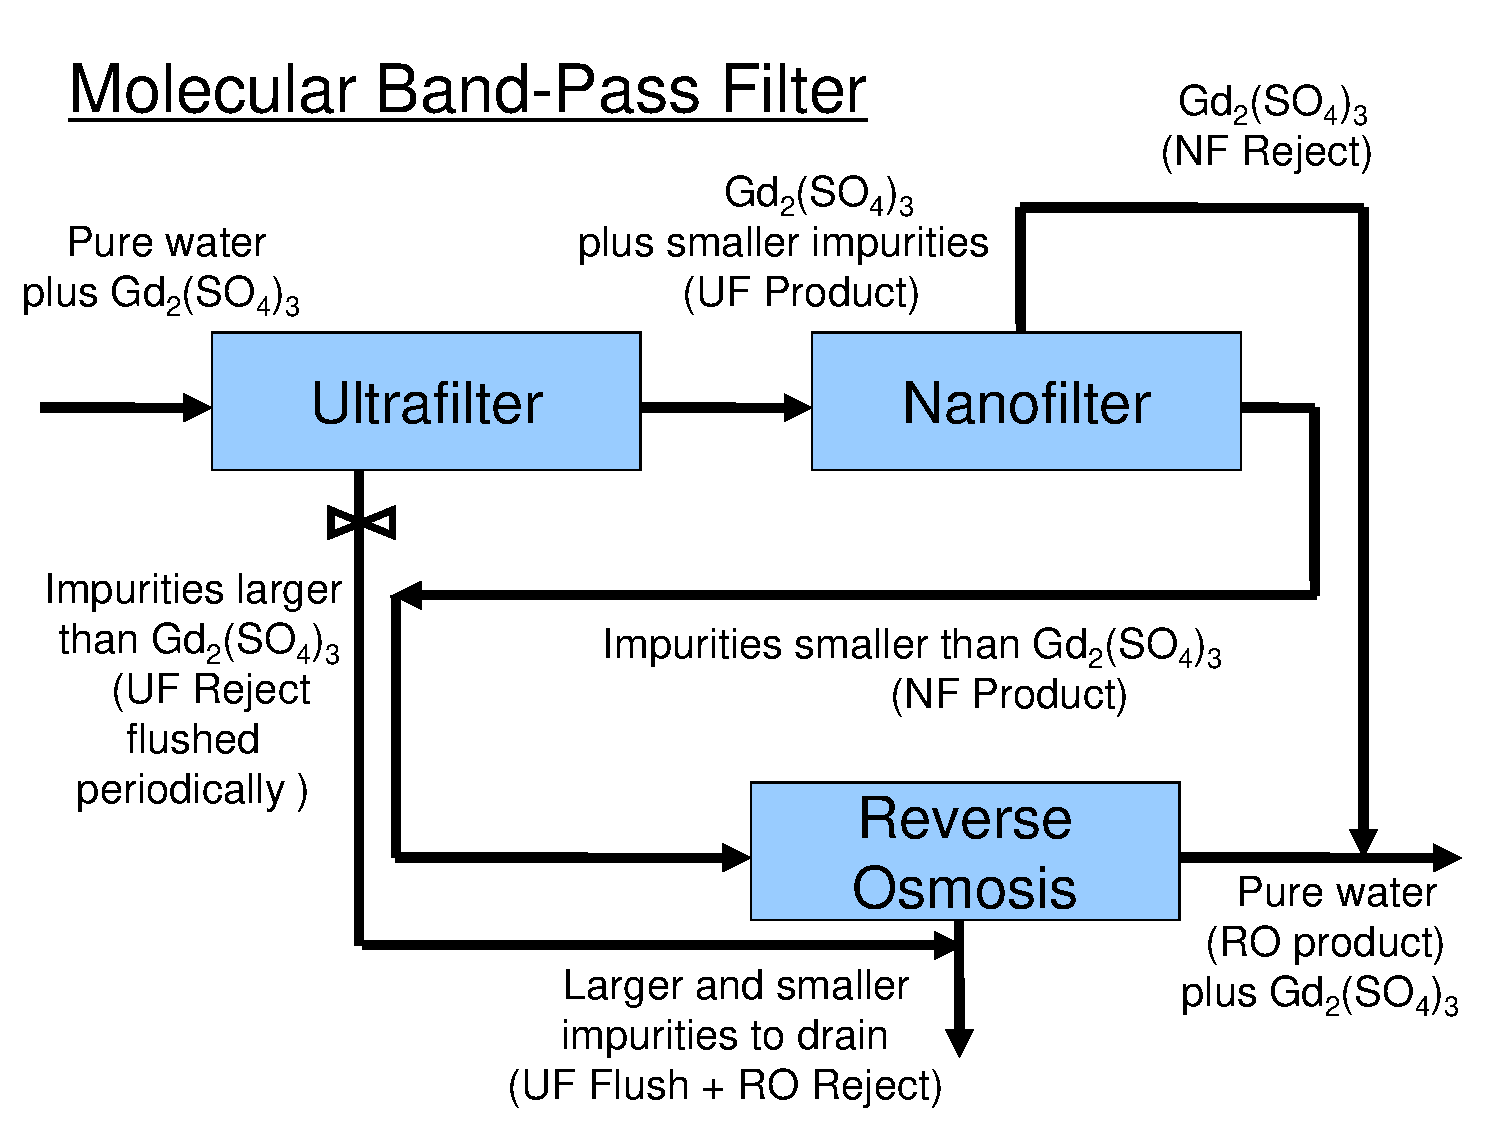
\includegraphics[width=9cm]{figures/nuPRISM_bandpass.pdf}
       \caption{A schematic illustration of the principle of the "molecular band-pass filter".  
       Successively fine filter elements isolate the dissolved gadolinium sulfate ions and return
       them to the main tank, bypassing water system elements which would be fouled if they 
       were to trap gadolinium.}
       \label{water:bandpass}
     \end{center}
\end{figure}


\clearpage

%\subsection{GPS \red{(Y. Hayato?)}}
%
%Section goals:
%\begin{itemize}
%\item Discussion of needed GPS system based on ND280 and recent GPS work
%\end{itemize}

